
% Chapter 3 File

\chapter{Database Construction: Reverse transcriptases from public databases}
\label{chapter2}
\thispagestyle{empty}



% \section{The origin of Retron data} 

% Current retron discovery suffers from a methodological bottleneck that perpetuates limited sequence diversity and hinders comprehensive characterization. The foundational work by Toro and colleagues [Ref. 8] employed term-based database searches and sequence similarity approaches to gather 198,760 entries, from which they identified 9,141 representative RT sequences and 17 representative groups including retrons (see Supplementary Figure 1). Notably, characterized retrons exhibit only ~25% average amino acid homology with each other and ~12-14% homology with specific other bacterial RT systems (such as Group II intron maturases and DGR RTs), highlighting their substantial sequence divergence [Ref. 12]. A following study identified 1,912 retron/retron-like sequences from the representative dataset, characterized retrons as a tripartite system, and subclassified them into clades based on accessory protein clustering and sequence similarity (see Supplementary Figure 2) [Ref. 9]. 


% ---------------------------------------------------------------
% Section: The origin of Retron data  (merged version)
% Requires: booktabs; natbib or biblatex
% Citation keys: toro2014, toro2018, toro2019, mestre2020,
%   kojima2008, simon2008, inouye1999, silas2017
% ---------------------------------------------------------------

\section{The origin of Retron data}
\label{sec:origin-retron-data}


% https://claude.ai/chat/7984ad47-4cb5-432d-9f1b-66d221c47a5d

% The retron sequence data available today originated not from a dedicated catalogue of retrons but
% from a series of progressively larger surveys of prokaryotic reverse transcriptases (RTs) as a
% whole, conducted over roughly six years by a single research group at the Estación Experimental
% del Zaidín (CSIC, Granada). Understanding what those surveys did, and equally what they did not
% attempt, is a prerequisite for interpreting any modern retron dataset, because the composition,
% the units of counting and the recall limits of every subsequent retron catalogue were fixed by
% decisions taken in them.
% \todo{enhance this sentence}
% Their design parameters and retron-relevant outcomes are summarised in
% Table~\ref{tab:rt-surveys}.

Current retron sequence data stems not from a dedicated retron catalogue, but from a six-year series of expanding prokaryotic reverse transcriptase (RT) surveys led by a single research group at the Estación Experimental del Zaidín (CSIC, Granada). Interpreting modern retron datasets requires understanding the boundaries of these foundational surveys, whose design decisions dictated the compositional bias, unit metrics, and recall limits of every subsequent collection. Table~\ref{tab:rt-surveys} summarizes their design parameters and retron-relevant outcomes.




\begin{table}[H]
\centering
\caption{Design Parameters and Retron-Relevant Outcomes of Foundational Prokaryotic Reverse Transcriptase Surveys}
\label{tab:rt-surveys}
\small
\begin{tabular}{@{}p{0.19\textwidth}p{0.24\textwidth}p{0.23\textwidth}p{0.26\textwidth}@{}}
\toprule
 & 
\textbf{Toro et al. (2014)} \cite{toro2014} & 
\textbf{Toro et al. (2018)} \cite{toro2018} & 
\textbf{Toro et al. (2019)} \cite{toro2019} \\
\midrule
Question &
How many coherent RT lineages exist in bacteria? &
Single or multiple origins for CRISPR-associated RTs? &
Comprehensive census of prokaryotic RTs and their genomic context \\
\addlinespace
Source &
PATRIC (RAST), complete genomes, 5 phyla &
Two published datasets, integrated &
PATRIC (2 queries), CDART, 2018 set, 6 manual additions \\
\addlinespace
Raw input & --- & --- & 198{,}760 sequences \\
\addlinespace
Final dataset & 742 sequences & 558 sequences & 9{,}141 representative RTs \\
\addlinespace
Filters &
$\geq$\,200 aa; 85\,\%; RT0--RT7 &
RT0--RT7 &
$\geq$\,200 aa; 85\,\%; RT0--RT7 \\
\addlinespace
Inference &
FastTree, RAxML &
FastTree (exploratory), IQ-TREE (definitive); ModelFinder/BIC; UFBoot, SH-aLRT &
FastTree, IQ-TREE; genomic-context pipeline (\texttt{hmmscan}, CRT, $\pm$30\,kb) \\
\addlinespace
Retron fraction &
13.7\,\% (102 sequences) &
Not assessed (retron RT used as outgroup) &
25\,\% (1{,}912 sequences) \\
\addlinespace
Basis of retron identification &
RT protein motifs only (VTG, 47\,\%; NAxxH, 59\,\%) &
--- &
RT protein motifs only; \textit{msr}/\textit{msd} absent in clade 14 \\
\addlinespace
ncRNA analysed? & No (stated explicitly) & No & No \\
\bottomrule
\end{tabular}
\begin{pbox}{\textwidth}
\vspace{4pt}
\scriptsize \textit{Note:} All sequence counts refer to representatives dereplicated at 85\,\% identity, not to loci or genomes.
\end{pbox}
\end{table}


% [EDITED] --- 2014 paragraph condensed; table rows no longer restated in prose.
\textit{Toro et al.} \cite{toro2014} conducted the first systematic genome-wide search for RTs across completely
sequenced bacterial genomes. Earlier BLAST-based surveys \cite{kojima2008, simon2008} had
already indicated that prokaryotic genomes harbour large numbers of uncharacterised RTs; the
authors' stated rationale for replacing homology search with an annotation harvest was the
uniform RAST annotation available through PATRIC, at the cost of restricting coverage to the
five phyla for which sufficient complete genomes then existed. The resulting 742-sequence
alignment (Table~\ref{tab:rt-surveys}) established a 17-group classification of bacterial RTs
--- group II introns, retrons/retron-like RTs, diversity-generating retroelements (DGRs),
Abi-like RTs, CRISPR-associated RTs, group II-like (G2L) RTs and eleven groups of unknown
function (UG1--UG11) --- in which group II intron ORFs dominated at approximately 57\,\%,
retrons followed at 13.7\,\% and DGRs at 8.4\,\%.

Three features of this study are material to everything that follows. First, the retron cluster
expanded to 102 representatives, an early indication that retrons were under-sampled rather than
genuinely rare.
\todo{verify the ``six previously known sequences'' claim against Toro \& Nisa-Martínez (2014);
by 2014 far more than six retrons had been described in the literature}
Second, the annotations retrieved for these sequences were strikingly inconsistent: entries were
variously labelled ``retron-type RNA-directed DNA polymerase'', ``mobile element protein'',
``hypothetical protein'' or simply ``reverse transcriptase'', and a conserved RT domain had to be
verified independently in each case regardless of how the entry had been annotated. Third, retron
identity was established entirely at the level of the RT protein, by two diagnostic motifs: the
VTG triplet within RT domain 7, in the region designated ``Y'', which mediates recognition of the
template-primer RNA used for msDNA synthesis \cite{inouye1999}, present in 47\,\% of sequences;
and the NAxxH motif in region ``X'' between domains 2 and 3, identifiable in 59\,\%. The authors
state explicitly that they made no attempt to identify msRNA or msDNA secondary structures. In
2014, a retron was therefore operationally defined as a position in an RT phylogeny accompanied by
a protein motif; the non-coding RNA that gives the element its function played no part in its
identification.
\todo{decide whether the 254 informative positions figure is correct --- the 2018 paper reports
250 positions over the same window}
\\

% [EDITED] --- 2018 paragraph: dataset provenance corrected, methods made concrete.
The second study, \cite{toro2018}, adjudicates between a single-acquisition model
\citep{silas2017} and repeated independent recruitment for the RTs adjacent to or fused with
Cas1 in type III CRISPR-Cas systems. Its dataset is not a survey of prokaryotic RTs but an
integration: the 537 sequences of \cite{toro2017}, of which 414 were group II intron RTs and 118
CRISPR-associated, plus 21 RT-like sequences reported by \cite{silas2017} and absent from that
set. Exactly one retron sequence appears in it, a retron-like RT from \textit{Haliscomenobacter
hydrossis} used to root the tree. The study therefore contributes no retron data; its importance
here is methodological, since it is where the pipeline later applied to retrons was assembled. It
established the use of FastTree for exploratory inference and IQ-TREE for the definitive tree,
with the substitution model (LG+G4) selected by ModelFinder under the Bayesian information
criterion and branch support estimated by ultrafast bootstrap (UFBoot), the SH-like approximate
likelihood ratio test (SH-aLRT, 1000 replicates) and standard non-parametric bootstrap (100
replicates), together with an explicit criterion for recognising a clade: FastTree local support
$\geq$\,0.9 combined with either non-parametric bootstrap $\geq$\,70\,\% or SH-aLRT and UFBoot
$\geq$\,80\,\%. It also supplies a caution worth carrying forward: for one node bearing directly
on the study's conclusion, FastTree local support (0.96) and the IQ-TREE metrics (SH-aLRT
53.5\,\%, UFBoot 67\,\%) disagreed, and non-parametric bootstrapping separated the clade
altogether. In RT phylogenies of this depth, the choice of support estimator can determine which
conclusion a tree appears to support.


% --- 2019 paragraph: unchanged from the original draft.
The scale of available data increased substantially with \cite{toro2019}, who assembled 198{,}760
sequences by combining PATRIC searches for proteins annotated as RNA-directed DNA polymerases
(145{,}379 entries) or reverse transcriptases (52{,}684 entries) with the previously published set
of 558 RT sequences, 133 RT-Cas1 fusion entries identified through conserved domain architecture
searches in CDART, and six further predicted RTs linked to type I-E CRISPR-Cas systems. After
extraction of the RT0--RT7 domain at a minimum length of 200 amino acids and clustering at 85\,\%
identity, the collection was reduced to 9{,}141 unique representative sequences, which remain the
reference dataset for the field (see Figure \ref{fig:toro_data}).
 
\todo{mention later that precise methodology on how they determined RT0-7 is not stated}
Group II introns account for 47\,\% of these, retron/retron-like
sequences for 25\,\%, and DGRs for 12\,\%. Broadening the corpus from complete genomes in five
phyla to complete and draft genomes across bacteria and archaea thus nearly doubled the retron
share relative to the 2014 census: retrons are the second most abundant class of reverse
transcriptase in the prokaryotic world.

\begin{figure}[H]
    \centering
    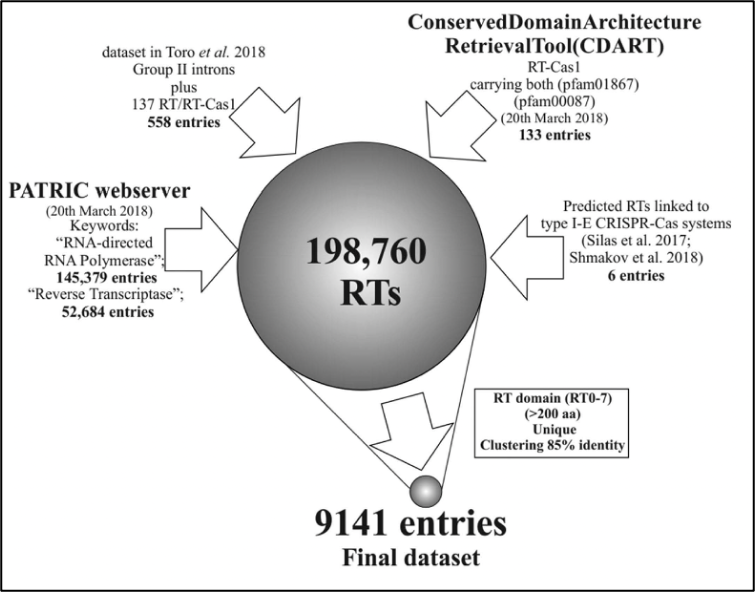
\includegraphics[width=0.8\textwidth]{Toro_data.png}  % Adjust width as needed for smaller image
    \caption{TBD.}
    \label{fig:toro_data}
\end{figure}


% --- Genomic-context / clade 14 paragraph: unchanged from the original draft.
This study was also the first in the series to characterise an RT by its genomic context rather
than by its own sequence. A dedicated pipeline annotated every gene within 30\,kb of each RT,
detected CRISPR arrays with CRT, and identified neighbouring proteins by \texttt{hmmscan} against a
composite profile database of CRISPR-Cas, effector and anti-phage defence models. Applied to
CRISPR-linked RTs, it demonstrated at least three independent evolutionary origins: the large
lineage derived from group II intron RTs, and two minor and more recent lineages derived
respectively from retron/retron-like RTs (clade 14) and from Abi-P2 RTs (clade 15). Both
previously competing models had assumed a single group II intron ancestry, and both were shown to
be incomplete. It is in the description of clade 14, however, that the study states the problem
that motivated everything after it: these RTs carry the canonical retron protein signatures, yet
no \textit{msr} and \textit{msd} genes could be identified in their vicinity. An RT may possess
every protein-level hallmark of a retron and nonetheless lack the component that defines the
element, because the non-coding RNA is invisible to protein-domain hidden Markov models.
Sequence-level homology to retron RTs does not by itself guarantee a complete, functional retron
locus.



These three studies bequeath three conventions and one gap. The conventions --- the RT0--RT7
window, the 200-amino-acid threshold and dereplication at 85\,\% identity --- are inherited
unexamined, and the last matters most: every count in this literature is of representative
sequences, not loci, retron systems or genomes, and cannot be compared with such counts without
explicit conversion. A fourth is never stated at all --- that the universe of prokaryotic RTs is
whatever public databases had already annotated as one --- a query the 2014 annotation
inconsistency shows to be leaky by an unquantified amount. The gap is the non-coding RNA: until
2020, retron identification rested on the reverse transcriptase alone. It was this dataset that
became the direct foundation of the first dedicated retron classification framework
\cite{mestre2020}.

% % [EDITED] --- closing paragraph: duplicated ncRNA and annotation material absorbed, wording tightened.
% Taken together, these studies bequeath to the work described in the following section three
% conventions and one gap. The conventions are the analytical window (RT domains 0 to 7), the
% minimum length threshold (200 amino acids) and the dereplication level (85\,\% identity), the last
% of which has a consequence easily overlooked: every published figure in this literature, from the
% 102 retron RTs of 2014 to the 9{,}141 representatives of 2019, counts representative sequences,
% not loci, retron systems or genomes, and cannot be compared with such counts without explicit
% conversion. A fourth convention is left unstated --- that the universe of prokaryotic RTs is
% operationally the set of sequences public databases had already annotated as reverse
% transcriptases --- and the annotation inconsistency noted above shows this query to miss genuine
% RTs without offering any estimate of how many. The gap, finally, is the absence of ncRNA evidence:
% until 2020, retron identification rested on the reverse transcriptase alone. It was this dataset
% that became the direct foundation of the first dedicated retron classification framework
% \cite{mestre2020}.


% \citet{toro2014} conducted the first systematic genome-wide search for RTs across completely
% sequenced bacterial genomes. Earlier surveys based on BLAST \citep{kojima2008, simon2008} had
% already indicated that prokaryotic genomes harbour large numbers of uncharacterised RTs, but were
% vulnerable to missing or incorrect homology assignments; 

% \todo{cross check these claims are true}
% the authors therefore replaced the
% homology search with an annotation harvest from the PATRIC platform, which provides uniform RAST
% annotation, restricted to the five phyla for which sufficient complete genomes were then
% available. Sequences shorter than 200 amino acids were discarded as probable fragments, the
% remainder dereplicated at 85\,\% identity, and the resulting set combined with a curated reference
% collection to give a final alignment of 742 sequences over the region corresponding to RT domains
% 0 to 7, yielding 254 informative positions for maximum-likelihood inference in FastTree and RAxML.
% The analysis established a 17-group classification of bacterial RTs --- group II introns,
% retrons/retron-like RTs, diversity-generating retroelements (DGRs), Abi-like RTs,
% CRISPR-associated RTs, group II-like (G2L) RTs and eleven groups of unknown function (UG1--UG11)
% --- in which group II intron ORFs dominated at approximately 57\,\%, retrons followed at
% 13.7\,\% and DGRs at 8.4\,\%.

% Three features of this study are material to everything that follows. First, the retron cluster
% grew from six previously known sequences to 102 representatives, an early indication that retrons
% were severely under-sampled rather than genuinely rare. Second, the annotations retrieved for
% these sequences were strikingly inconsistent: entries were variously labelled ``retron-type
% RNA-directed DNA polymerase'', ``mobile element protein'', ``hypothetical protein'' or simply
% ``reverse transcriptase'', and a conserved RT domain had to be verified independently in each case
% regardless of how the entry had been annotated. This is the first clear signal that keyword-based
% database queries are insufficient for reliably recovering RT and retron sequences --- a
% limitation inherited, unquantified, by every dataset built on the same approach. Third, retron
% identity was established entirely at the level of the RT protein, by two diagnostic motifs: the
% VTG triplet within RT domain 7, in the region designated ``Y'', which mediates recognition of the
% template-primer RNA used for msDNA synthesis \citep{inouye1999}, present in 47\,\% of sequences;
% and the NAxxH motif in region ``X'' between domains 2 and 3, identifiable in 59\,\%. The authors
% state explicitly that they made no attempt to identify msRNA or msDNA secondary structures. In
% 2014, a retron was therefore operationally defined as a position in an RT phylogeny accompanied by
% a protein motif; the non-coding RNA that gives the element its function played no part in its
% identification.

% The second study, \citet{toro2018}, concerns RTs adjacent to or fused with Cas1 in type III
% CRISPR-Cas systems, and adjudicates between a single-acquisition model \citep{silas2017} and
% repeated independent recruitment. A retron RT appears in it only as the outgroup used to root the
% tree, so it contributes no retron data; its importance here is methodological, since it is where
% the pipeline later applied to retrons was assembled. It established the use of FastTree for
% exploratory inference and IQ-TREE for the definitive tree, with the substitution model selected by
% ModelFinder under the Bayesian information criterion and branch support estimated by both
% ultrafast bootstrap (UFBoot) and the SH-like approximate likelihood ratio test (SH-aLRT), together
% with an explicit criterion for recognising a clade. It also supplies a caution worth carrying
% forward: for one node bearing directly on the study's conclusion, FastTree local support (0.96)
% and the IQ-TREE metrics (SH-aLRT 53.5\,\%, UFBoot 67\,\%) disagreed, and non-parametric
% bootstrapping separated the clade altogether. In RT phylogenies of this depth, the choice of
% support estimator can determine which conclusion a tree appears to support.

% The scale of available data increased substantially with \citet{toro2019}, who assembled 198{,}760
% sequences by combining PATRIC searches for proteins annotated as RNA-directed DNA polymerases
% (145{,}379 entries) or reverse transcriptases (52{,}684 entries) with the previously published set
% of 558 RT sequences, 133 RT-Cas1 fusion entries identified through conserved domain architecture
% searches in CDART, and six further predicted RTs linked to type I-E CRISPR-Cas systems. After
% extraction of the RT0--RT7 domain at a minimum length of 200 amino acids and clustering at 85\,\%
% identity, the collection was reduced to 9{,}141 unique representative sequences, which remain the
% reference dataset for the field (see Figure \ref{fig:toro_data}). 

% \todo{mention later that precise methodology on how they determined RT0-7 is not stated}
% Group II introns account for 47\,\% of these, retron/retron-like
% sequences for 25\,\%, and DGRs for 12\,\%. Broadening the corpus from complete genomes in five
% phyla to complete and draft genomes across bacteria and archaea thus nearly doubled the retron
% share relative to the 2014 census: retrons are not a peripheral curiosity but the second most
% abundant class of reverse transcriptase in the prokaryotic world.


% \begin{figure}[H]
%     \centering
%     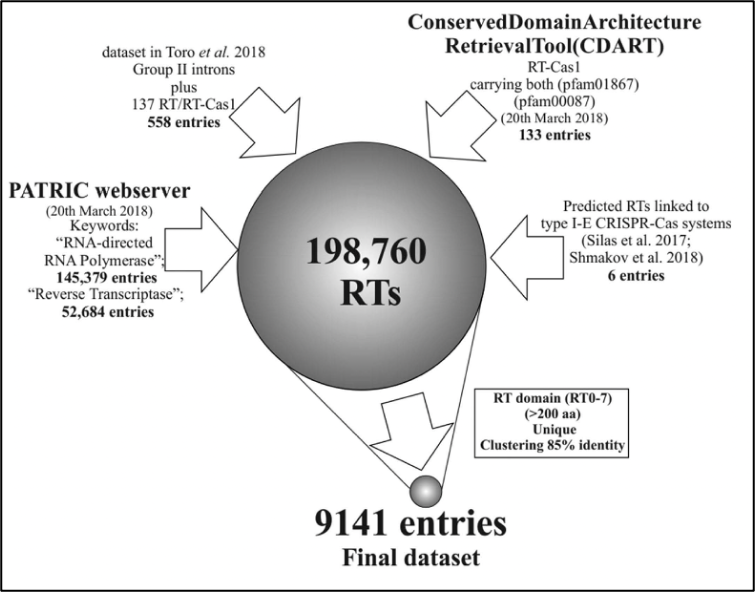
\includegraphics[width=0.8\textwidth]{Toro_data.png}  % Adjust width as needed for smaller image
%     \caption{TBD.}
%     \label{fig:toro_data}
% \end{figure}


% This study was also the first in the series to characterise an RT by its genomic context rather
% than by its own sequence. A dedicated pipeline annotated every gene within 30\,kb of each RT,
% detected CRISPR arrays with CRT, and identified neighbouring proteins by \texttt{hmmscan} against a
% composite profile database of CRISPR-Cas, effector and anti-phage defence models. Applied to
% CRISPR-linked RTs, it demonstrated at least three independent evolutionary origins: the large
% lineage derived from group II intron RTs, and two minor and more recent lineages derived
% respectively from retron/retron-like RTs (clade 14) and from Abi-P2 RTs (clade 15). Both
% previously competing models had assumed a single group II intron ancestry, and both were shown to
% be incomplete. It is in the description of clade 14, however, that the study states the problem
% that motivated everything after it: these RTs carry the canonical retron protein signatures, yet
% no \textit{msr} and \textit{msd} genes could be identified in their vicinity. An RT may possess
% every protein-level hallmark of a retron and nonetheless lack the component that defines the
% element, because the non-coding RNA is invisible to protein-domain hidden Markov models.
% Sequence-level homology to retron RTs does not by itself guarantee a complete, functional retron
% locus.

% Taken together, these three studies bequeath to the work described in the following section three
% conventions and one gap. The conventions are the analytical window (RT domains 0 to 7), the
% minimum length threshold (200 amino acids) and the dereplication level (85\,\% identity), the last
% of which has a consequence easily overlooked: every published figure in this literature, from the
% 102 retron RTs of 2014 to the 9{,}141 representatives of 2019, counts representative sequences,
% not loci, retron systems or genomes, and cannot be compared with such counts without explicit
% conversion. A fourth convention is left unstated --- that the universe of prokaryotic RTs is
% operationally the set of sequences public databases had already annotated as reverse
% transcriptases --- and the annotation inconsistency noted above shows this query to miss genuine
% RTs without offering any estimate of how many. The gap, finally, is the absence of ncRNA evidence:
% until 2020, retron identification rested on the reverse transcriptase alone. It was this dataset
% that became the direct foundation of the first dedicated retron classification framework
% \citep{mestre2020}.

% ---------------------------------------------------------------





% https://claude.ai/chat/228c3edb-7ea5-43b7-a0e5-e9844c7dd295


% The retron sequence data available today originated from a series of progressively larger bacterial reverse transcriptase (RT) surveys rather than from a single comprehensive catalog. Toro and Nisa-Martínez (2014) conducted the first systematic genome-wide search for RTs across all completely sequenced bacterial genomes, establishing a 17-group classification of bacterial RTs that included retrons/retron-like sequences as a distinct lineage; within this study, the retron-associated cluster grew from just six previously known sequences to 102 representative sequences sharing $\le$85\% identity, marking the first formal expansion of the retron sequence space beyond a handful of experimentally characterized examples. Notably, the annotations retrieved for these sequences were highly inconsistent — entries were variously labeled as ``retron-type RNA-directed DNA polymerase,'' ``mobile element protein,'' ``hypothetical protein,'' or simply ``reverse transcriptase'' — and a conserved RT domain had to be independently verified in each case regardless of how it had been annotated, an early indication that keyword-based database searches alone are insufficient for reliably identifying RT and retron sequences. A subsequent study examining RTs linked to CRISPR-Cas systems (Toro et al., 2018) reinforced that retron-like RTs form a recognizable, evolutionarily distinct lineage, identifiable by conserved sequence motifs even when found outside canonical retron loci. The scale of available data increased substantially with Toro et al. (2019), who assembled a dataset of 198,760 sequences by combining PATRIC database searches for proteins annotated as RNA-directed DNA polymerases (145,379 entries) or reverse transcriptases (52,684 entries) with a previously published set of 558 RT sequences, 133 RT-Cas1 fusion entries identified via conserved domain architecture searches, and six additional predicted RTs linked to type I-E CRISPR-Cas systems. After extracting the conserved RT domain (RT0–7, $\ge$200 amino acids) from each entry and clustering these domain sequences at 85\% identity, this collection was reduced to 9,141 unique representative sequences, of which approximately 25\% (roughly 2,285 sequences) were classified as retron or retron-like — the largest single contributor to RT diversity after group-II introns. Phylogenetic reconstruction of this representative dataset, combined with screening for CRISPR-Cas gene neighborhoods, revealed that retron/retron-like sequences represent one of at least three independent evolutionary origins of RTs subsequently captured by CRISPR-Cas systems. In at least one such case, the identified RT carried retron-diagnostic sequence motifs but lacked any detectable msr/msd genes — the non-coding RNA component that defines a functional retron — in its genomic neighborhood, indicating that sequence-level homology to retron RTs does not by itself guarantee the presence of a complete, functional retron locus. This dataset would later serve as the direct foundation for the first dedicated retron classification framework (Mestre et al., 2020).

% The retron sequence data available today originated from a series of progressively larger bacterial reverse transcriptase (RT) surveys rather than from a single comprehensive catalog. Toro and Nisa-Martínez (2014) conducted the first systematic genome-wide search for RTs across all completely sequenced bacterial genomes, establishing a 17-group classification of bacterial RTs that included retrons/retron-like sequences as a distinct lineage; within this study, the retron-associated cluster grew from just six previously known sequences to 102 representative sequences sharing $\le$85\% identity, marking the first formal expansion of the retron sequence space beyond a handful of experimentally characterized examples. A subsequent study examining RTs linked to CRISPR-Cas systems (Toro et al., 2018) reinforced that retron-like RTs form a recognizable, evolutionarily distinct lineage, identifiable by conserved sequence motifs even when found outside canonical retron loci. The scale of available data increased substantially with Toro et al. (2019), who assembled a dataset of 198,760 sequences by combining PATRIC database searches for proteins annotated as RNA-directed DNA polymerases (145,379 entries) or reverse transcriptases (52,684 entries) with a previously published set of 558 RT sequences, 133 RT-Cas1 fusion entries identified via conserved domain architecture searches, and six additional predicted RTs linked to type I-E CRISPR-Cas systems. After extracting the conserved RT domain (RT0–7, $\ge$200 amino acids) from each entry and clustering these domain sequences at 85\% identity, this collection was reduced to 9,141 unique representative sequences, of which approximately 25\% were classified as retron or retron-like — the largest single contributor to RT diversity after group-II introns. Phylogenetic reconstruction of this representative dataset, combined with screening for CRISPR-Cas gene neighborhoods, revealed that retron/retron-like sequences represent one of at least three independent evolutionary origins of RTs subsequently captured by CRISPR-Cas systems. This dataset would later serve as the direct foundation for the first dedicated retron classification framework (Mestre et al., 2020). 





\section{Current Retron Classification}
\label{sec:current-classification}


Building on the reverse-transcriptase dataset described in the previous section, Rodríguez Mestre
et al.\ set out to determine whether bacterial retrons extend beyond the canonical two-component
(ncRNA\,+\,RT) element, and to place the resulting systems within an explicit evolutionary
framework \cite{mestre2020}. Their prior was a long-standing observation: roughly one third of
annotated retrons carry additional open reading frames, variously annotated as adenosine-binding
or cold-shock proteins or not annotated at all, whose role in retron biology was unresolved. The
input dataset is not new --- it is the 9{,}141 representative sequences of \cite{toro2019}, from
which the 1{,}912 retron/retron-like sequences were extracted and supplemented with 16 RTs from
experimentally validated retrons compiled by \cite{simon2019}, giving the 1{,}928 sequences
analysed. What is new is the question, and the constraint the authors imposed on themselves in
answering it: the test for association was to be free of bias with respect to the phylogenetic
group of the RT, the genomic context of the RT gene, the distance to the RT gene, and any
hypothesis about the accessory gene's function.
 

The study rests on four analyses that, although often summarised together as ``phylogenetic and
co-evolutionary'', are distinct in both method and statistical power; their tools, parameters and
outcomes are set out in Table~\ref{tab:mestre-methodology}. They are also logically dependent on
one another. Analysis (a) reconstructs a reverse-transcriptase phylogeny and thereby establishes
the clade structure that serves as the organising axis for everything that follows; (b) and (c)
map the two other candidate components --- the cognate \textit{msr}--\textit{msd} non-coding RNA
and a third, protein-coding or RT-fused component --- onto that axis; and (d) asks whether the
three evolve as a unit rather than as a recurrent coincidence. Together they provide systematic
evolutionary evidence \textit{supporting} a tripartite and modular architecture, in which an
\textit{msr}--\textit{msd}--RT core acquires diverse effector modules.
 
\subsection{(a) The reverse-transcriptase phylogeny}
 
A maximum-likelihood phylogeny of the conserved RT0--RT7 region resolved eleven clades whose
internal nodes exceed 85\,\% support under both metrics (Table~\ref{tab:mestre-methodology}). All
sequences displayed the retron RT features described in Section~\ref{sec:origin-retron-data}:
region Y at the C-terminus, containing the VTG triplet within RT7 and directing the RT to its
cognate \textit{msr}; and region X, between RT2 and RT3, bearing the NAxxH motif.
 
Two properties of this tree matter for what follows. First, in contrast to group II introns and
DGRs, retron RT phylogenies are well resolved even at internal nodes, which the authors interpret
as evidence of comparatively recent diversification --- a favourable circumstance for any
subsequent phylogenetic work on this family, and the implicit justification for treating these
clades as a stable framework onto which the remaining components can be mapped. Second, of the
eleven clades only six contained an experimentally validated retron: five of the clades that
organise the entire classification have no characterised representative whatsoever.


\subsection{(b) Recovery of the non-coding RNA component}
 
The second analysis addressed the ncRNA gap left open in 2019, by two routes. Where an
experimentally confirmed \textit{msr}--\textit{msd} transcript was available, it was used as a seed
to build covariance models, with which the regions flanking each RT gene were searched for
comparable structures. Where no validated seed existed, structured regions were instead sought by
manual secondary-structure inspection, aligned in a structure-aware mode to identify conserved
elements in closely related genomes, and the search iterated. In both routes the proposed
consensus structures were finally tested for covarying base pairs, which reduces the weight of
phylogenetic correlation and base-composition bias and thereby distinguishes genuine structural
conservation from mere sequence similarity.
 
Canonical structures were recovered with confidence in eight of the eleven clades, including
clades with no previously validated representative; no significant consensus could be obtained for
clades 4, 5 and 6 (per-clade detail in Table~\ref{tab:clade-coverage}). The authors are careful to
note that failure to recover a canonical structure does not itself demonstrate the absence of an
ncRNA.


\subsection{(c) A statistical test for non-random gene association}
 
The third analysis is the study's methodological core. All ORFs flanking each RT were retrieved
and clustered, and a presence/absence matrix constructed in which rows corresponded to the RTs
ordered by their position in the phylogenetic tree and columns to the neighbouring protein
clusters. Note that the ORF search was run across the full set of 9{,}141 representative RTs
rather than the retron-like subset alone, since the controls described below require the
CRISPR-associated, DGR and group II intron RTs to be present.
 
Two filters were then applied in succession. The first, the \textit{phyvalue}, formalises the
expectation that a functionally associated cluster should occupy a phylogenetically contiguous
block rather than being scattered at random: it is a moving average down each column, normalised
against the moving average and standard deviation of size-matched random permutations of that
column. The second filter addresses the confounder that the first cannot --- neighbouring genes
will appear phylogenetically clustered simply because closely related RTs occur in closely related
genomes. Requiring that the RTs sharing a given neighbour be less than 60\,\% identical demands
that the association survive across divergent genomes, where it cannot be attributed to recent
common ancestry. Candidates fell from 131 to 71 subclusters, which were then curated manually and
reannotated.
 
The controls deserve particular emphasis, since they are the reason the result can be believed. As
positive controls, the pipeline correctly recovered Cas2 in the neighbourhood of CRISPR-associated
RTs and the Avd protein in the neighbourhood of DGRs, both independently established
associations. As a negative control, the clusters neighbouring group II introns scored 94.56\,\%
on phylogenetic accumulation --- that is, they passed the first filter convincingly --- and then
failed the sequence-identity test, exactly as would be expected of autonomous mobile retroelements
that carry no functional partner gene. The negative control was therefore capable of failing and
did not, which is what demonstrates that the second filter performs genuine discrimination rather
than merely restating the first.
 
Function was assigned to the surviving clusters by three independent routes: remote homology
detection with domain assignment, \textit{de novo} structural modelling, and structural homology
transfer by searching the resulting models against the Protein Data Bank
(Table~\ref{tab:mestre-methodology}). Throughout, the authors check whether the catalytic residues
implied by an assignment are actually present, and record explicitly where they are not.


\subsection{(d) Co-evolution of the three components}
 
That the three components constitute a functional unit rather than a recurrent coincidence was
addressed by comparing independently inferred phylogenies of the RT, the associated protein and
the ncRNA of each system, against a 16S rRNA phylogeny of the hosts as a control for the
underlying speciation background (Table~\ref{tab:mestre-methodology}). RT distances correlated
strongly with associated-protein distances in every type examined, consistent with direct and
specific protein--protein interaction; the correlation between the RT and the ncRNA was also
strong, though slightly weaker, which the authors interpret as indicating a broader mechanistic
role for the ncRNA. Correlation with the host 16S phylogeny was weak or absent in all types except
XIII ($\approx$\,0.78), which alone appears to be vertically inherited, consistent with earlier
reports from the Myxobacteria.

\subsection{(b) Recovery of the non-coding RNA component}
 
The second analysis addressed the ncRNA gap left open in 2019. Using each experimentally confirmed
\textit{msr}--\textit{msd} transcript and its close relatives as a seed, the authors ran CMfinder
v0.4.1 to predict RNA motifs from a combination of folding energy and sequence covariation, built
covariance models with Infernal, and searched the regions flanking each RT gene for comparable
structures. Where no validated seed existed, structured regions were sought manually with RNAfold,
aligned with the structure-aware MAFFT Q-INS-i mode to identify conserved elements in closely
related genomes, trimmed at the complementary a1 and a2 termini, and the search iterated. R-scape
was then applied to identify covarying base pairs in the proposed consensus structures, reducing
the weight of phylogenetic correlation and base-composition bias and thereby distinguishing
genuine structural conservation from mere sequence similarity.
 
Canonical structures were recovered with confidence in eight of the eleven clades, including
clades with no previously validated representative. Clades 7 and 8 each yielded a single consensus
structure, whereas clades 1, 2, 3, 9, 10 and 11 yielded two or three distinct structures apiece;
no significant consensus could be obtained for clades 4, 5 and 6. The authors are careful to note
that failure to recover a canonical structure does not itself demonstrate the absence of an ncRNA.


% ---------------------------------------------------------------
% Table 2: methodological framework
% ---------------------------------------------------------------
 
\begin{table}[H]
\centering
\scriptsize
\setlength{\tabcolsep}{4pt}
\renewcommand{\arraystretch}{1.25}
\begin{threeparttable}
\caption[Methodological framework of Rodríguez Mestre et al.]{Methodological framework used by Mestre et al.
\cite{mestre2020} to establish the current retron classification. Tool versions and parameters
are reported only where explicitly stated by the authors, and are \textit{n.s.}\ (``not stated''
in the source) unless given. The consequences of these omissions are taken up in
Section~\ref{sec:classification-limitations}.}
\label{tab:mestre-methodology}
\begin{tabularx}{\textwidth}{
    >{\raggedright\arraybackslash}p{0.13\textwidth}
    >{\raggedright\arraybackslash}p{0.27\textwidth}
    >{\raggedright\arraybackslash}p{0.27\textwidth}
    >{\raggedright\arraybackslash}X}
\toprule
\textbf{Analysis} & \textbf{Methods and tools} & \textbf{Key parameters and criteria} &
\textbf{Main result} \\
\midrule
 
\textbf{(a) RT phylogeny} &
Alignment of the conserved RT0--RT7 regions (MAFFT, mode \textit{n.s.}\ for this analysis), model
selection with ModelFinder, maximum-likelihood inference with IQ-TREE v1.6.12.\tnote{a} &
1{,}912 retron/retron-like RTs plus 16 experimentally validated retrons (1{,}928 tips). LG+F+R10
(lowest BIC of 546 models). Support from 1{,}000 UFBoot and 1{,}000 SH-aLRT replicates; nodes
deemed well supported when both exceed 85\,\%. No alignment trimming reported. &
\textbf{11 well-supported clades}, with the 16 validated retrons distributed across 6 of them.
Clade delimitation followed from node support rather than an explicit algorithmic rule. \\
\addlinespace
 
\textbf{(b) ncRNA (\textit{msr}--\textit{msd})} &
A seeded route used CMfinder v0.4.1 on validated transcripts to build covariance models
(Infernal), searched around the RT loci. Where seeds were unavailable, candidates were identified
by manual secondary-structure inspection (RNAfold), aligned with MAFFT Q-INS-i, and iteratively
refined. Structural signal was tested with R-scape. &
Search radius around the RT \textit{n.s.} In the unseeded route, the stopping criterion for
iterative refinement was \textit{n.s.}, and R-scape statistical power was not reported. The a1/a2
hybridisation region was trimmed during alignment. &
Confident consensus structures for \textbf{8 of the 11 RT clades}; none for clades 4--6; types
VIII and XI lack a recognisable canonical ncRNA module. Per-clade detail in
Table~\ref{tab:clade-coverage}. \\
\addlinespace
 
\textbf{(c) Third component} &
ORFs flanking each RT were clustered with MMseqs2 (connected-component clustering followed by
iterative cascaded profile searches to convergence) and tested for non-random association across
the RT phylogeny using the custom \textit{phyvalue} statistic. Surviving associations were
manually curated and reannotated with MAFFT and HMMER, then functionally characterised by
remote-homology and structure-based prediction.\tnote{b} &
ORFs of 30--3{,}000\,aa within $\pm$30\,kb of each RT; 62{,}277 clusters (5{,}413 with $>$5
members). \textit{phyvalue}: bandwidth 50, step 1, cutoff $=$ mean $+$ 4\,SD over 10{,}000
permutations, ratio $\geq$\,2; clusters split at runs of $>$10 sub-threshold positions. A further
filter required $<$60\,\% RT identity between associated systems. Positive controls: Cas2 at
CRISPR-associated RTs, Avd at DGRs. Negative control: group II introns, which passed the
\textit{phyvalue} filter at 94.56\,\% and were then eliminated by the identity filter. Number of
subclusters removed during manual curation \textit{n.s.} &
Candidates reduced from \textbf{131} to \textbf{71 associated protein subclusters}, supporting the
definition of \textbf{13 retron system types} (with subtypes and variants). Associated components
are not confined to single RT clades, indicating substantial modularity. \\
\addlinespace
 
\textbf{(d) Co-evolution} &
Independent phylogenies for the RT, ncRNA and associated protein (MAFFT FFT-NS-i or Q-INS-i;
IQ-TREE) compared by cophenetic-distance correlation (R 3.6, \texttt{dendextend}). Host
evolutionary history represented by a 16S rRNA phylogeny (SILVA). &
Restricted to types with $\geq$\,20 representatives; IQ-TREE under default settings with 1{,}000
bootstrap replicates. No null model, confidence interval or significance estimate reported for the
correlations. &
RT--protein correlations generally strong, RT--ncRNA strong but somewhat weaker, correlation with
the host 16S phylogeny generally weak or absent --- type XIII the exception
($\approx$\,0.78). The authors interpret this as \textit{suggesting} coordinated evolution of the
components beyond shared host ancestry. \\
\bottomrule
\end{tabularx}
\begin{tablenotes}[flushleft]\footnotesize
\item[a] FastTree (WAG, 20 rate categories) was the default for the study's exploratory trees; the
RT phylogeny of (a) and the co-evolution trees of (d) were built with IQ-TREE.
\item[b] HHpred and HHblits with InterPro, Pfam and SMART for remote homology and domains;
RaptorX, Phyre2, I-TASSER and trRosetta for structure modelling; DALI and PDBeFold for fold
matching.
\end{tablenotes}
\end{threeparttable}
\end{table}

 


\subsection{Retrons as tripartite, modular systems}
 
On this basis the study advances its central claim: that retrons are tripartite systems composed
of the (\textit{msr}-\textit{msd}) non-coding RNA, the reverse transcriptase, and a third
component --- either an associated protein-coding gene or a domain fused to the C-terminus of the
RT --- and that retron systems can be classified into thirteen types, several with subtypes or
variants, according to the identity of that third component. The classification is given in
Table~\ref{tab:retron-types}.
 
The classification also reveals pronounced modularity. The same (\textit{msr}-\textit{msd})-RT
cassette may be associated with different effectors --- types I-A and II-A1 share clade 1 RTs and
a common ncRNA structure family yet recruit an ATPase and an NDT respectively --- while conversely
the same effector function recurs alongside distantly related RTs, as with the PRTases found in
clades 2, 5, 6 and 9. Stand-alone cassettes lacking any associated protein occur in clades 2 and
11. The authors accordingly propose that the ncRNA and RT together constitute a sensing or
recognition module, and the associated protein a response module, exchanged under selective
pressure from rapidly evolving phages. This interpretation was corroborated almost immediately:
work published within weeks \cite{gao2020, millman2020} demonstrated experimentally that retron
types I-A, II-A3, I-C1 and XII mediate anti-phage defence, and that the additional protein or
RT-fused domain is required for that activity.
 
The two outputs most relevant to the present work are the reverse-transcriptase phylogeny and the
resulting system classification, both reproduced in Figure~\ref{fig:mestre-tree}. Panel~A shows
the eleven RT clades that define the evolutionary framework of analysis (a), with the
experimentally characterised retrons labelled and the clades distinguished by colour; panel~B
translates the effector-based analysis of (c) into a schematic of the thirteen retron system
types, coloured to match their parent RT clades. Their juxtaposition makes explicit the point that
governs how this classification should be read: the eleven clades and the thirteen types are two
different objects, produced by two different pipelines. The clades derive from RT sequence alone,
whereas the types are defined by the associated effector, so the type-level classification is, by
construction, not congruent with the RT phylogeny. This deliberate incongruence is the clearest
expression of the modularity described above, and it is the framework that the present thesis sets
out to re-examine at larger scale and under an explicitly phylogeny-controlled approach.
 

% ---------------------------------------------------------------
% Table: the thirteen types
% ---------------------------------------------------------------
 
\begin{table}[H]
\centering
\caption[Classification of retron systems]{Classification of retron systems after
\cite{mestre2020}. Types are defined by the identity of the third component, which is either a
separate open reading frame or a domain fused to the RT C-terminus. The fifteen rows correspond to
thirteen types, since I-B, I-C, II-A, III-A and VII-A comprise subtypes of a single type. Clade
numbers refer to the eleven-clade RT phylogeny. A dash indicates a type with no experimentally
characterised representative at the time of publication.}
\label{tab:retron-types}
\scriptsize
\renewcommand{\arraystretch}{1.15}
\begin{tabular}{@{}>{\raggedright\arraybackslash}p{0.09\textwidth}
                  >{\raggedright\arraybackslash}p{0.08\textwidth}
                  >{\raggedright\arraybackslash}p{0.44\textwidth}
                  >{\raggedright\arraybackslash}p{0.29\textwidth}@{}}
\toprule
Type & RT clade & Third component & Validated representatives \\
\midrule
I-A & 1 & ABC ATPase (Walker A/B, P-loop NTPase) with HNH endonuclease & Eco7 (Ec78), Eco4 (Ec83),
Vpa1 (Vp96), Vch1 (Vc95) \\
I-B1, I-B2 & 1, 3 & ABC ATPase with TOPRIM domain & --- \\
I-C1--C3 & 8 & TOPRIM domain fused to the RT C-terminus & Eco2 (Ec67) \\
II-A1--A3 & 1, 1, 9 & Nucleoside deoxyribosyltransferase-like (NDT) with C-terminal DNA-binding
domain & Sen2 (St85), Vch2 (Vc81), Eco3 (Ec73), Eco1 (Ec86), Vch3 (Vc137) \\
III-A1--A5 & 2, 5, 6, 9 & Phosphoribosyltransferase-like (PRTase), alone or with a winged-helix
auxiliary protein & --- \\
IV & 3 & Integral membrane protein (signal peptide, two TM helices) & Eco6 (Ec48) \\
V & 3 & Cold-shock DNA-binding domain protein & Sen1 (Se72) \\
VI & 3 & Cro/C1-type HTH protein with accessory proteins of epsilon-antitoxin-like fold & --- \\
VII-A1, VII-A2 & 4 & DUF3800, fused or free; structurally RNase H2-like & --- \\
VIII & 4 & Putative serine esterase (DUF626) & --- \\
IX & 7 & HEPN domain protein with winged-helix DNA-binding partner & --- \\
X & 7 & IHF-like DNA-binding domain with C-terminal VHL-like domain & --- \\
XI & 8 & Trypsin-like serine protease fused to the RT C-terminus & --- \\
XII & 8 & TIR-2 domain fused to the RT C-terminus & --- \\
XIII & 10 & SWIM Zn-finger protein with transposase-like DEDE motif, preceded by HEAT/ARM-repeat
proteins & Nex2 (Ne144), Mxa1 (Mx162), Mxa2 (Mx65), Sau1 (Sa163) \\
\bottomrule
\end{tabular}
\end{table}



 
% ---------------------------------------------------------------
% Figure
% ---------------------------------------------------------------
 
\begin{figure}[H]
\centering
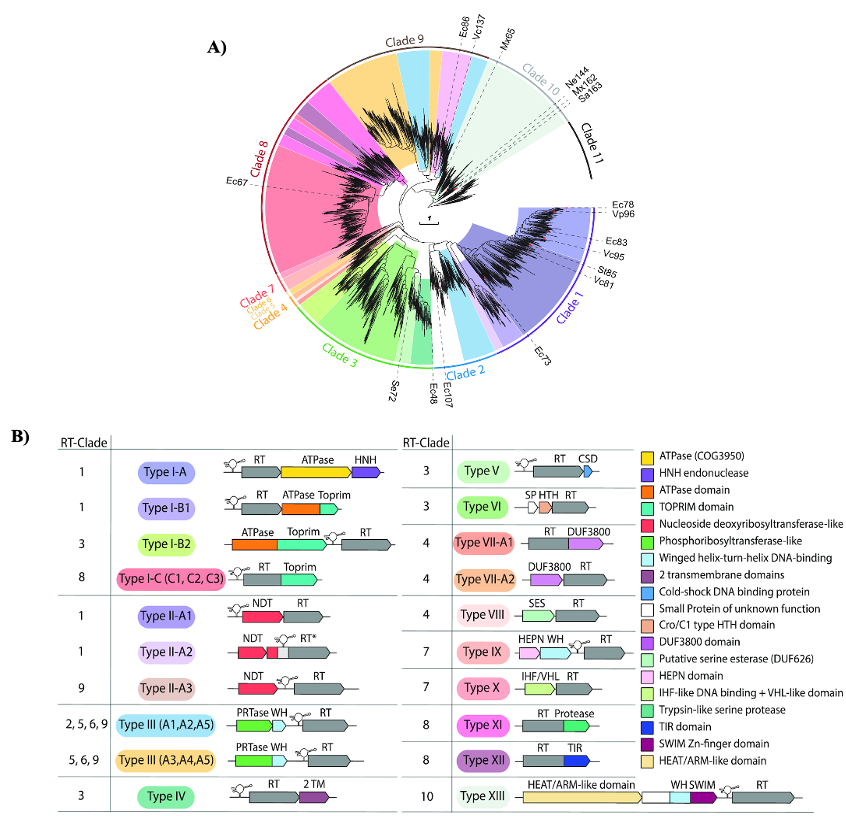
\includegraphics[width=\textwidth]{MESTRE_tree_and_retron_operons.png}
\caption[Evolutionary and structural diversity of retron systems]{Evolutionary and structural
diversity of retron systems. (A)~Phylogenetic reconstruction of retron and retron-like reverse
transcriptases. Major clades, indicated by coloured lines and outer rings, provide the
organising axis of the classification; RTs from experimentally characterised retrons are
labelled. (B)~Schematic representation of retron system architectures, classifying the types and
variants by genomic organisation, with colours corresponding to the RT clades in panel~A.
Reproduced from \citet{mestre2020} under CC~BY~4.0.}
\label{fig:mestre-tree}
\end{figure}


% \section{Current Retron Classification-claude1}
% \label{sec:current-classification}
 
% The classification in use today derives from a single study, \citet{mestre2020}, which is best
% understood as the point at which the general-purpose RT survey described in the preceding section
% was turned upon retrons themselves. Its input dataset is not new: it is the 9{,}141 representative
% sequences of \citet{toro2019}, from which the 1{,}912 sequences classified as retron/retron-like
% were extracted and supplemented with 16 RTs from experimentally validated retrons compiled by
% \citet{simon2019}, giving the 1{,}928 sequences analysed. What is new is the question.
% Approximately one third of annotated retrons were known to carry additional open reading frames,
% variously annotated as adenosine-binding or cold-shock proteins or not annotated at all, whose
% significance was undetermined. The authors asked whether these accessory genes are functionally
% associated with the retron or merely happen to lie nearby, and imposed on themselves an explicit
% design constraint: the test was to be free of bias with respect to the phylogenetic group of the
% RT, the genomic context of the RT gene, the distance to the RT gene, and any hypothesis about the
% accessory gene's function. Answering it required three separate analyses, and the study's
% principal contribution is that it delivered all three.
 
% \subsection{A resolved phylogeny of retron reverse transcriptases}
 
% A multiple sequence alignment of the RT0--RT7 region of the 1{,}928 retron RT sequences was
% constructed with MAFFT and analysed in IQ-TREE v1.6.12 under the LG+F+R10 substitution model,
% identified by ModelFinder as having the lowest Bayesian information criterion among 546 candidate
% protein models, with branch support estimated from 1{,}000 ultrafast bootstrap replicates and
% 1{,}000 SH-aLRT replicates. The analysis resolved eleven well-supported clades, whose internal
% nodes exceed 85\,\% support under both metrics. The authors note that, in contrast to group II
% introns and DGRs, retron RT phylogenies are well resolved even at internal nodes, which they
% interpret as evidence of comparatively recent diversification --- a favourable circumstance for
% any subsequent phylogenetic work on this family. All sequences displayed the characteristic
% retron RT features described in Section~\ref{sec:origin-retron-data}: region Y, at the C-terminus,
% containing the VTG triplet within RT7 and directing the RT to its cognate \textit{msr}; and region
% X, between RT2 and RT3, bearing the NAxxH motif. Of the eleven clades, only six contained an
% experimentally validated retron; five had no characterised representative whatsoever.
 
% \subsection{Recovery of the non-coding RNA component}
 
% The second analysis addressed the ncRNA gap left open in 2019. Using each experimentally confirmed
% \textit{msr}-\textit{msd} transcript and its close relatives as a seed, the authors ran CMfinder
% 0.4.1 to predict RNA motifs from a combination of folding energy and sequence covariation, built
% covariance models with Infernal, and searched the regions upstream and downstream of each RT gene
% for comparable structures. Where no validated seed existed, structured regions were sought
% manually with RNAfold, aligned with the structure-aware MAFFT Q-INS-i mode to identify conserved
% elements in closely related genomes, trimmed at the complementary a1 and a2 termini, and the
% search iterated. R-scape was then applied to identify covarying base pairs in the proposed
% consensus structures, reducing the weight of phylogenetic correlation and base-composition bias
% and thereby distinguishing genuine structural conservation from mere sequence similarity.
 
% By this route, canonical \textit{msr}-\textit{msd} structures were recovered with confidence in
% eight of the eleven clades, including clades with no previously validated representative. Clades 7
% and 8 each yielded a single consensus structure, whereas clades 1, 2, 3, 9, 10 and 11 yielded two
% or three distinct structures apiece. No significant consensus structure could be obtained for
% clades 4, 5 and 6.
 
% \subsection{A statistical test for non-random gene association}
 
% The third analysis is the study's methodological core. All open reading frames within 30\,kb
% upstream and downstream of each of the 9{,}141 RTs were retrieved and clustered with MMseqs2,
% discarding sequences shorter than 30 or longer than 3{,}000 amino acids, using connected-component
% clustering followed by iterative cascaded profile searches until convergence in order to capture
% remote homologues. This produced 62{,}277 clusters, of which 5{,}413 contained more than five
% members. A presence/absence matrix was then constructed in which rows corresponded to the RTs
% ordered by their position in the phylogenetic tree and columns to the neighbouring protein
% clusters, on the reasoning that a functionally associated cluster should occupy a phylogenetically
% contiguous block rather than being scattered at random.
 
% Two filters were applied in succession. The first, which the authors term the \textit{phyvalue},
% is computed as a moving average down each column (bandwidth 50, step 1) normalised against the
% moving average and standard deviation of 10{,}000 size-matched random permutations, with the
% significance threshold set at the permutation mean plus four standard deviations and a requirement
% that the maximum ratio reach two; clusters were further divided into subclusters wherever more
% than ten consecutive positions fell below the threshold. This reduced the candidates to 131
% subclusters. The second filter addresses the confounder that the first cannot: neighbouring genes
% will appear phylogenetically clustered simply because closely related RTs occur in closely related
% genomes. The authors therefore required that the RTs sharing a given neighbour have less than
% 60\,\% sequence identity, that is, that they be sufficiently divergent for the shared neighbour
% not to be attributable to recent common ancestry. This reduced the set to 71 subclusters, which
% were then curated manually and re-annotated using MAFFT alignments and HMMER profiles.
 
% The controls deserve particular emphasis, since they are the reason the result can be believed. As
% positive controls, the pipeline correctly recovered Cas2 in the neighbourhood of CRISPR-associated
% RTs and the Avd protein in the neighbourhood of DGRs, both independently established associations.
% As a negative control, the clusters neighbouring group II introns scored 94.56\,\% on phylogenetic
% accumulation --- that is, they passed the first filter convincingly --- and then failed the
% sequence-identity test, exactly as would be expected of autonomous mobile retroelements that carry
% no functional partner gene. The negative control was therefore capable of failing and did not,
% which is what demonstrates that the second filter performs genuine discrimination rather than
% merely restating the first.
 
% Function was assigned to the surviving clusters by a consistent three-stage procedure: remote
% homology detection with HHpred and HHblits and domain assignment with InterPro, Pfam and SMART;
% independent structural modelling with RaptorX, Phyre2, I-TASSER and trRosetta; and structural
% homology transfer by searching the resulting models against the Protein Data Bank with DALI and
% PDBeFold. Throughout, the authors check whether the catalytic residues implied by an assignment
% are actually present, and record explicitly where they are not.
 
% \subsection{Retrons as tripartite systems}
 
% On this basis the study advances its central claim: that retrons are tripartite systems composed
% of the (\textit{msr}-\textit{msd}) non-coding RNA, the reverse transcriptase, and a third
% component --- either an associated protein-coding gene or a domain fused to the C-terminus of the
% RT --- and that retron systems can be classified into thirteen types, several with subtypes or
% variants, according to the identity of that third component. The classification is given in
% Table~\ref{tab:retron-types}.
 
% That these three components constitute a functional unit rather than a recurrent coincidence was
% established by coevolution analysis. Independent phylogenies were inferred for the RT, the
% associated protein and the ncRNA of each system, and their branch-length distance matrices
% compared by cophenetic correlation, using 16S rRNA trees retrieved from SILVA as a control for the
% underlying speciation background and restricting the analysis to types for which at least twenty
% complete systems could be assembled. RT distances correlated strongly with associated-protein
% distances in every type examined, consistent with direct and specific protein--protein
% interaction; the correlation between the RT and the ncRNA was also strong, though slightly weaker,
% which the authors interpret as indicating a broader mechanistic role for the ncRNA. Correlation
% with the host 16S rRNA was negligible in all types except XIII, which alone appears to be
% vertically inherited, consistent with earlier reports from the Myxobacteria.
 
% The classification also revealed pronounced modularity. The same (\textit{msr}-\textit{msd})-RT
% cassette may be associated with different effectors --- types I-A and II-A1 share clade 1 RTs and
% a common ncRNA structure family yet recruit an ATPase and an NDT respectively --- while
% conversely the same effector function recurs alongside distantly related RTs, as with the PRTases
% found in clades 2, 5, 6 and 9. Stand-alone cassettes lacking any associated protein occur in
% clades 2 and 11. The authors accordingly propose that the ncRNA and RT together constitute a
% sensing or recognition module, and the associated protein a response module, exchanged under
% selective pressure from rapidly evolving phages. This interpretation was corroborated almost
% immediately: work published within weeks \citep{gao2020, millman2020} demonstrated experimentally
% that retron types I-A, II-A3, I-C1 and XII mediate anti-phage defence, and that the additional
% protein or RT-fused domain is required for that activity.
 
% % ---------------------------------------------------------------
 
% \begin{table}[H]
% \centering
% \caption[Classification of retron systems]{Classification of retron systems after
% \citet{mestre2020}. Types are defined by the identity of the third component, which is either a
% separate open reading frame or a domain fused to the RT C-terminus. Clade numbers refer to the
% eleven-clade RT phylogeny. A dash in the final column indicates a type with no experimentally
% characterised representative at the time of publication.}
% \label{tab:retron-types}
% \small
% \renewcommand{\arraystretch}{1.15}
% \begin{tabular}{@{}>{\raggedright\arraybackslash}p{0.09\textwidth}
%                   >{\raggedright\arraybackslash}p{0.08\textwidth}
%                   >{\raggedright\arraybackslash}p{0.44\textwidth}
%                   >{\raggedright\arraybackslash}p{0.29\textwidth}@{}}
% \toprule
% Type & RT clade & Third component & Validated representatives \\
% \midrule
% I-A & 1 & ABC ATPase (Walker A/B, P-loop NTPase) with HNH endonuclease & Eco7 (Ec78), Eco4 (Ec83),
% Vpa1 (Vp96), Vch1 (Vc95) \\
% I-B1, I-B2 & 1, 3 & ABC ATPase with TOPRIM domain & --- \\
% I-C1--C3 & 8 & TOPRIM domain fused to the RT C-terminus & Eco2 (Ec67) \\
% II-A1--A3 & 1, 1, 9 & Nucleoside deoxyribosyltransferase-like (NDT) with C-terminal DNA-binding
% domain & Sen2 (St85), Vch2 (Vc81), Eco3 (Ec73), Eco1 (Ec86), Vch3 (Vc137) \\
% III-A1--A5 & 2, 5, 6, 9 & Phosphoribosyltransferase-like (PRTase), alone or with a winged-helix
% auxiliary protein & --- \\
% IV & 3 & Integral membrane protein (signal peptide, two TM helices) & Eco6 (Ec48) \\
% V & 3 & Cold-shock DNA-binding domain protein & Sen1 (Se72) \\
% VI & 3 & Cro/C1-type HTH protein with accessory proteins of epsilon-antitoxin-like fold & --- \\
% VII-A1, VII-A2 & 4 & DUF3800, fused or free; structurally RNase H2-like & --- \\
% VIII & 4 & Putative serine esterase (DUF626) & --- \\
% IX & 7 & HEPN domain protein with winged-helix DNA-binding partner & --- \\
% X & 7 & IHF-like DNA-binding domain with C-terminal VHL-like domain & --- \\
% XI & 8 & Trypsin-like serine protease fused to the RT C-terminus & --- \\
% XII & 8 & TIR-2 domain fused to the RT C-terminus & --- \\
% XIII & 10 & SWIM Zn-finger protein with transposase-like DEDE motif, preceded by HEAT/ARM-repeat
% proteins & Nex2 (Ne144), Mxa1 (Mx162), Mxa2 (Mx65), Sau1 (Sa163) \\
% \bottomrule
% \end{tabular}
% \end{table}



% \section{Current Retron Classification-MELISSA} 



% Building on the reverse-transcriptase dataset described in the previous section, Rodríguez Mestre et al.\ set out to determine whether bacterial retrons extend beyond the canonical two-component (ncRNA + RT) element, and to place the resulting systems within an explicit evolutionary framework. Their study rests on four analyses that, although often summarized together as ``phylogenetic and co-evolutionary'', are distinct in both method and statistical power; these are set out in Table~\ref{tab:rodriguez_mestre_methodology}. The first (a) reconstructs a reverse-transcriptase phylogeny from the conserved RT0--7 regions of 1,928 sequences, resolving eleven well-supported clades that serve as the organizing axis for everything that follows. Onto this axis the remaining analyses map the two other candidate components: (b) a structure-based search recovers the cognate \emph{msr--msd} non-coding RNA, confidently in eight of the eleven clades; and (c) a statistical association pipeline---built on ORF clustering and the custom \emph{phyvalue} statistic rather than on a protein phylogeny---identifies a third, protein-coding or RT-fused component and reduces tens of thousands of neighbouring clusters to seventy-one functionally associated subclusters. Finally, (d) a co-evolution analysis compares the independently inferred RT, ncRNA and protein trees against a host 16S rRNA control, and reports that the components' evolutionary histories are correlated more strongly with one another than with host ancestry. Taken together, these analyses provide systematic evolutionary evidence \emph{supporting} a tripartite and modular architecture, in which an \emph{msr--msd}--RT core acquires diverse effector modules.

% % Building on the prokaryotic RT dataset introduced earlier, Mestre et al. set out to test whether retrons are more than a two-part (ncRNA + RT) element. Their prior was the long-standing observation that roughly one third of annotated retrons carry additional ORFs of unknown function, whose role in retron biology was unresolved. They analysed 1,912 retron/retron-like RT sequences (plus 16 experimentally validated retrons) and concluded that retrons are generally tripartite systems: the (msr-msd) ncRNA, the RT, and a third associated protein-coding gene or an RT-fused domain.



% % Following the systematic identification of retron reverse transcriptases described above, Rodríguez Mestre et al. sought to determine whether retrons could be systematically organized according to the evolutionary relationships between their constituent components. Their analysis was based on 1,912 retron or retron-like reverse transcriptases, complemented by 16 experimentally validated retrons, and focused on three main questions: how retron RTs are evolutionarily related, which non-coding and protein-coding components are associated with these RTs, and whether these components exhibit evidence of coordinated evolution. Rather than defining retrons solely from the presence of an RT, the authors therefore considered the genomic and evolutionary context surrounding each RT to establish a system-level classification.



% \begin{table}[H]
% \centering
% \scriptsize
% \setlength{\tabcolsep}{4pt}
% \renewcommand{\arraystretch}{1.25}
% \caption{Methodological framework used by Rodríguez Mestre et al.\ to establish the
% current retron classification. Tool versions and parameters are reported only where
% explicitly stated by the authors; \emph{n.s.}\ denotes ``not stated'' in the source.}
% \label{tab:rodriguez_mestre_methodology}
% \begin{tabularx}{\textwidth}{
%     >{\raggedright\arraybackslash}p{0.14\textwidth}
%     >{\raggedright\arraybackslash}p{0.29\textwidth}
%     >{\raggedright\arraybackslash}p{0.29\textwidth}
%     >{\raggedright\arraybackslash}X
% }
% \hline
% \textbf{Analysis} &
% \textbf{Methods and tools} &
% \textbf{Key parameters and criteria} &
% \textbf{Main result} \\
% \hline

% \textbf{RT phylogeny}
% &
% Multiple sequence alignment of the conserved RT0--7 regions (MAFFT, mode \emph{n.s.}\
% for this analysis), model selection with ModelFinder, and maximum-likelihood inference
% with IQ-TREE v1.6.12.
% &
% 1,912 retron/retron-like RTs plus 16 experimentally validated retrons (1,928
% tips).\footnotemark[1] Model LG+F+R10 (lowest BIC of 546 models). Support from 1,000
% ultrafast bootstrap and 1,000 SH-aLRT replicates; nodes deemed well supported when both
% exceeded 85\%. No alignment trimming reported.
% &
% \textbf{11 well-supported clades}, with the 16 validated retrons distributed across 6 of
% them. These clades provided the evolutionary framework onto which the ncRNA and protein
% components were subsequently mapped. Clade delimitation followed from node support rather
% than an explicit algorithmic rule.
% \\

% \hline

% \textbf{ncRNA (msr--msd)}
% &
% A seeded route used CMfinder v0.4.1 on experimentally validated transcripts to build
% covariance models (Infernal), searched around the RT loci. Where seeds were unavailable,
% candidate ncRNAs were identified by manual secondary-structure inspection (RNAfold),
% aligned with MAFFT Q-INS-i, and iteratively refined. Conserved structural signal was
% tested with R-scape.\footnotemark[2]
% &
% Search radius around the RT \emph{n.s.} In the unseeded route, the stopping criterion for
% iterative refinement was \emph{n.s.}, and R-scape statistical power was not reported. The
% a1/a2 hybridization region was trimmed during alignment.
% &
% Confident consensus structures for \textbf{8 of the 11 RT clades}; some clades carried two
% or three structural variants, whereas no convincing consensus was found for clades 4--6,
% and types VIII and XI lacked a recognizable canonical ncRNA module. The authors noted that
% failure to recover a canonical structure did not itself demonstrate absence of an ncRNA.
% \\

% \hline

% \textbf{Third component}
% &
% ORFs flanking each RT were clustered with MMseqs2 (version \emph{n.s.}) and tested for
% non-random association across the RT phylogeny using the custom \emph{phyvalue} statistic.
% Surviving associations were manually curated and reannotated with HMMER, then functionally
% characterized by remote-homology and structure-based
% prediction.\footnotemark[3]
% &
% ORFs of 30--3,000\,aa within $\pm$30\,kb of each RT; 62,277 clusters (5,413 with $>$5
% members). \emph{phyvalue}: bandwidth 50, cutoff = mean $+$ 4\,SD over 10,000 permutations,
% ratio $\geq 2$. A further filter required $<$60\% RT identity between associated systems.
% Positive control: RT--CRISPR/Cas2; negative control: group~II introns.
% &
% Candidates were reduced from \textbf{131} to \textbf{71 associated protein subclusters},
% supporting the definition of \textbf{13 retron system types} (with subtypes/variants).
% Associated components were not confined to single RT clades, indicating substantial
% modularity of the tripartite system.
% \\

% \hline

% \textbf{Co-evolution}
% &
% Independent phylogenies for the RT, ncRNA, and associated protein (MAFFT FFT-NS-i or
% Q-INS-i; IQ-TREE\footnotemark[4]) were compared by cophenetic-distance correlation
% (R 3.6, \texttt{dendextend}). Host evolutionary history was represented by a 16S rRNA
% phylogeny (SILVA).
% &
% Restricted to types with $\geq$20 representatives; IQ-TREE run under default settings with
% 1,000 bootstrap replicates. No null model, confidence interval, or significance estimate
% was reported for the correlations.
% &
% RT--protein correlations were generally strong and RT--ncRNA correlations strong but
% somewhat weaker, whereas correlation with the host 16S phylogeny was generally weak or
% absent---type XIII being the exception ($\approx$0.78). The authors interpreted this as
% \emph{suggesting} coordinated evolution of the components beyond shared host ancestry.
% \\

% \hline
% \end{tabularx}
% \footnotetext[1]{The 1,912 retron/retron-like RTs derive from a set of 9,141
% representative sequences clustered at 85\% identity from 198,760 annotated prokaryotic RTs
% (Toro et al.\ 2019); see Section~\ref{sec:XXX}. The final set is essentially
% bacterial.\footnotemark[5]}
% \footnotetext[2]{R-scape distinguishes covariation due to conserved structure from
% phylogenetic and compositional background, and was applied to every proposed consensus.}
% \footnotetext[3]{HHpred/HHblits and InterPro, Pfam and SMART for remote homology and
% domains; RaptorX, Phyre2, I-TASSER and trRosetta for structure modelling; DALI and
% PDBeFold for fold matching. Version numbers were \emph{n.s.}\ for all of these.}
% \footnotetext[4]{The paper's default for other trees is FastTree (WAG, 20 rate
% categories); the co-evolution trees are the stated exception, built with IQ-TREE.}
% \footnotetext[5]{1,899 Bacteria, no Archaea, and 29 unclassified entries.}
% \end{table}

% % \vspace{1mm}
% % \begin{minipage}{0.95\textwidth}
% % \footnotesize
% % \textit{Note:} n.s., not stated in the source paper.
% % \end{minipage}
% % \end{table}





% The two outputs most relevant to the present work are their reverse-transcriptase phylogeny and the resulting system classification, both reproduced in Figure~\ref{fig:metre_tree}. Panel~A shows the eleven RT clades that define the evolutionary framework of analysis (a), with the experimentally characterized retrons labelled and the clades distinguished by colour; panel~B translates the effector-based analysis of (c) into a schematic of the thirteen retron system types, coloured to match their parent RT clades. The juxtaposition makes explicit a point that is central to how this classification should be read: the eleven clades and the thirteen types are two different objects, produced by two different pipelines. The clades derive from RT sequence alone, whereas the types are defined by the associated effector; because functionally similar effectors recur across distantly related clades---and a single clade can carry several distinct effector types---the type-level classification is, by construction, not congruent with the RT phylogeny. This deliberate incongruence is the clearest expression of the modularity the authors describe, and it is the framework that the present thesis sets out to re-examine at larger scale and under an explicitly phylogeny-controlled approach.





\section{Traditional methods for discovery and annotation or retrons} 


Detection and classification of homologous proteins in large-scale genomic and metagenomic data relies heavily on profile hidden Markov models (HMMs), which act as statistical templates of a protein family. Built from a multiple sequence alignment of known family members, a profile HMM encodes position-specific emission and transition probabilities across match, insert, and delete states for each alignment column. This structure allows the model to capture exactly which residues are conserved, which positions tolerate substitution, and where insertions or deletions are evolutionarily permitted. Because this framework is generative and probabilistic, query sequences are evaluated against the model using likelihood-based scoring schemes rather than simple pairwise identity. This enables the highly sensitive detection of remote homologs that share a conserved domain architecture, even when overall sequence identity is exceptionally low—a property that has made profile HMM methods, such as those implemented in the HMMER software suite \cite{krogh1994hmm, eddy2011hmmer}, central to modern homology search and reference database curation \cite{mistry2021pfam}.

Covariance models (CMs) extend this probabilistic concept by incorporating information about conserved secondary structure and correlated nucleotide substitutions, making them particularly powerful for the identification of structured non-coding RNAs \cite{eddy1994covariance, durbin1998biological}. This formalism is implemented in the Infernal package \cite{nawrocki2013infernal}, which is used among others to build and search the Rfam database of structured RNA families \cite{kalvari2021rfam}. In genome-scale analyses, coding sequences are first predicted from assembled contigs using gene-calling tools such as Prodigal \cite{hyatt2010prodigal} or FragGeneScan \cite{rho2010fraggenescan}, which identify putative open reading frames and translate them into protein sequences. These predicted proteins can then be screened against curated HMM databases using software such as HMMER, while structural RNA elements are identified using Infernal. 

These approaches are nonetheless constrained by the knowledge used to build them.
A profile can only be constructed from an alignment of already-characterised
family members, so genuinely novel or highly divergent families remain invisible
until a first representative is identified by other means; iterative and
profile--profile strategies extend sensitivity but do not remove this dependency
\cite{remmert2012hhblits}. Detection is also bounded by the upstream gene call,
as short, overlapping or non-canonically initiated open reading frames are
routinely missed by \textit{ab initio} predictors, particularly on fragmented
metagenomic contigs \cite{sberro2019small}. Finally, a significant hit reports
membership of a profile rather than a specific biological function, so
domain-level homology alone is often insufficient to assign a system to a
particular pathway. The combination of accurate gene prediction and profile-based homology detection forms the basis of numerous annotation pipelines and specialized tools for identifying complex biological systems, including prokaryotic antiviral defense mechanisms. 


\todo{add a schematic of HHM/CMs?}

% The following tools were selected for demonstrating state-of-the-art performance and being widely employed for system annotation and classification in novel genomes. Rather than relying on a single method, we implemented a parallelized integration of all three tools, combining their outputs to substantially increase overall sensitivity and capture divergent homologs missed by any one program alone:\\



% \begin{wrapfigure}{l}{0.25\textwidth}
%   
\includegraphics[width=\linewidth]{myrt_logo.png}
% \end{wrapfigure}




% \textbf{MyRT}, is the first comprehensive tool for classifying bacterial reverse transcriptases (RTs), going beyond simple detection to assign each RT into one of 41 functional classes. The tool employs a three-layer architecture built on 45 class-specific HMMs derived from 1,988 curated RT sequences. Detection proceeds in two stages: an initial fast scan flags candidate RTs using a combined HMM model (e-value $<$ 10$^{-4}$), after which a comprehensive domain-validation step searches candidates against a large pre-existing reference library (\textasciitilde{}59,000 CDD/Pfam-A domains) to discard false positives lacking genuine RT-related domains. Verified RTs are also searched by BLASTP against a curated reference collection of known RTs to identify their closest homolog. Class assignment is then made directly when one class clearly dominates the hits; only low-confidence or unclassified candidates undergo phylogenetic placement via pplacer onto a reference RT tree. Finally, MyRT examines the genomic neighborhood of each RT (up to $\pm$4 genes, within a 2,000 bp intergenic distance, also searched against the CDD/Pfam-A library) to refine classifications --- for instance, reassigning RVT-CRISPR to RVT-CRISPR-like when no nearby cas genes are detected --- based on domain co-occurrence frequencies rather than a fixed mandatory/accessory/forbidden architecture. This approach achieves 90--100\% accuracy across test sets.

% The platform's database contains 43 class-specific HMM profiles covering all bacterial RT types, including 2 Group II intron profiles (GII-I, GII-II), 5 CRISPR-Cas profiles (G1-G5), 1 DGR profile, 1 retron profile, 7 abortive infection profiles (AbiA, AbiK, AbiP2, G2L variants), and 28 uncharacterized groups (UG1-UG28), plus CRISPR-like variants. Specifically, for retrons, the database contains a single HMM profile (RVT-Retrons), built from 91 retron RT sequences spanning 191 amino acid positions of the RVT\_1 domain, curated from multiple sources including Toro et al. (2019) [Ref. 8] and systematically validated through phylogenetic analysis.


% \\


% \begin{wrapfigure}{l}{0.25\textwidth}
%   
\includegraphics[width=\linewidth]{defense_finder_logo.png}
% \end{wrapfigure}

% \textbf{DefenseFinder}, is a comprehensive detection platform designed to identify known antiviral systems in prokaryotic genomes with high sensitivity and specificity. Built upon the MacSyFinder v2 framework for complex macromolecular systems, the tool employs a two-step strategy: it first uses profile HMMs to identify potential defense-associated proteins, and then applies system-specific decision rules to evaluate their genetic architecture. To minimize false positives, these rules categorize detected proteins into mandatory components required for function, accessory components that may be present, or forbidden components that are strictly excluded from the system structure. This rigorous architectural validation ensures that proteins are not evaluated in isolation, achieving up to 99.4\% sensitivity and 99.97\% specificity.

% The platform is capable of detecting 152 defense systems across 264 subtypes using 845 curated HMM profiles with optimized gathering thresholds. Specifically, for retrons, the database contains 15 HMM profiles for reverse transcriptase variants (Retron\_\_RT\_Tot\_1 through \_15) plus \textasciitilde{}30 additional profiles for accessory genes across 13 Retron subtypes (I\_A, I\_B, I\_C, II, III, IV, V, VI, VII\_1, VII\_2, VIII, IX, X, XI, XII, XIII). Each subtype is governed by strict co-occurrence rules that dictate the exact combination of mandatory genes required---such as the NDT and RT\_Tot pairing in Retron\_II---while systematically excluding forbidden genetic arrangements to accurately define the system boundaries based on foundational literature. Mestre et al (2020) [Ref. 9] and Millman et al.[Ref. 1]. 


% \begin{wrapfigure}{l}{0.25\textwidth}
%   
\includegraphics[width=\linewidth]{padloc-logo.png}
% \end{wrapfigure}


% \textbf{PADLOC}, is a defense-system annotation platform designed to identify and classify antiviral defense systems in bacterial and archaeal genomes. PADLOC searches for complete defense systems by integrating protein homology detection with system-level architecture analysis. It operates by scanning proteins genomes profile Hidden Markov Models (HMMs) to detect potential defense-related proteins. The tool evaluates their genomic organization against predefined system models (YAML files), which map out the genetic architecture of specific defense systems (within $\le$3 genes separation). In these files, proteins are categorized as core (essential for function), optional (not strictly required), or prohibited (used to differentiate between closely related systems that share similar components). PADLOC filters putative defense genes, groups them into clusters based on their genomic proximity (controlled by a maximum separation parameter), and checks if they meet the minimum required thresholds for core and total genes reducing false positives to <1\% while maintaining >97\% recall.


% Its database contains approximately 3,500 HMMs spanning more than 700 protein families across 180 system types, sourced and benchmarked from foundational defense system studies including Millman et al., Mestre et al., Gao et al., and Payne et al. For retrons, the database features 18 distinct system types (Types I-A, I-B, I-C, II-A, III-A, IV, V, VI, VII-A1, VII-A2, VIII, X, XI, XII, XIII, Ec107-like, outgroup, plus single-gene variants), utilizing 65 specialized HMM profiles targeting reverse transcriptases and effector proteins alongside 21 Infernal covariance models (CMs) designed for non-coding RNA (ncRNA) detection and phylogenetic classification across RT-Clades 1–10. 


% While each tool employs unique synteny criteria and profile-building strategies, they all rely heavily on the same foundational source data established by del Toro, Mestre et al., supplemented by additional experimental work. This shared foundation is both a strength and a limitation: while it ensures consistency where tools agree, it offers no independent arbiter when they disagree. Thus, distinguishing true positives from algorithmic artifacts remains an open challenge that ultimately demands orthogonal experimental confirmation.


\section{Large Scale Mining for bacterial retrons and RTs} 


The general workflow for the discovery and annotation of novel retron systems is
depicted in Figure~\ref{fig:retron-workflow}. The foundational survey of
\cite{mestre2020}, discussed in Section~\ref{sec:current-classification}, established both the
framing of the task and much of the methodological toolkits still in use ---
profile HMMs for the reverse transcriptase, covariance models for the
\textit{msr--msd}, and the phylogenetic scaffold onto, with 11 well-supported clades and 13 functional types based on their accessory modules, which subsequent candidates
are mapped.


It also established something that later work has repeatedly borne
out: that these tools do not run to completion unattended when no ncRNA molecule is found by the CM profiles. Their own definition
of the \textit{msr--msd} boundaries in clades without an experimentally validated
transcript rested on manual inspection of candidate folds and on iterative
refinement of the alignments, with trimming of the a1 and a2 arms and re-extraction
of the flanking sequence repeated until a consensus structure emerged. Manual
curation is not a fallback in this workflow but a constituent step.

% The same pattern is visible in a study spanning sampling, computational analysis
% and functional testing of retrons from environmental isolates
% \cite{nakamura2025}. There, PADLOC recovered retron operons from
% most 
% \todo{is most the correct word?}
% sequenced genomes but returned nothing for two of nine, leaving open
% whether the responsible loci lay in poorly covered regions, belonged to an
% uncharacterised subtype, or were not retrons at all. In a further case the
% predicted non-coding RNA proved incomplete once RT-DNA sequencing reads were
% found to map beyond the predicted boundary, and the annotation had to be revised
% against experimental evidence. Where PADLOC failed outright, candidate RTs were
% recovered instead by DefenseFinder and BLAST, and the surrounding genes assigned
% by combining their orientation with functional predictions from BLAST and
% InterPro. The characterisation of Retron-Sda1 in that same work makes the
% underlying limitation explicit: retron diversity extends past the thirteen
% recognised subtypes, and systems whose operons resist classification are
% precisely those that motif-based annotators are least able to find. For these,
% the RT gene remains the only dependable point of entry.


The same pattern is visible in a study combining environmental sampling, computational analysis and functional testing of retrons \cite{nakamura2025}. Because candidate systems were first identified through the physical detection of RT-DNA, the authors could recognise active retrons even where computational annotation was incomplete. PADLOC predicted complete retron operons in five of the seven identified hosts and recovered a lone retron RT in a sixth. Where it failed to identify the remaining system, Retron-Bth1, the candidate RT was instead recovered through manual inspection of DefenseFinder HMMER hits and a broader search for RTs using MyRT \todo{this comes from the final uploaded paper! we basically thought of the same}. Experimental evidence also exposed limitations at the ncRNA level, with RT-DNA sequencing used to refine the boundaries and predicted structures of the reverse-transcribed regions. Retron-Bth1 provides the clearest example of the underlying problem: its RT is interrupted by a group II intron and the system lacks an obvious canonical effector, features that make it poorly represented by the architectures assumed by existing annotation models. Together with Retron-Sda1, it could not be assigned to the established retron types. Thus, the study illustrates how divergent retrons can escape or remain incomplete under automated annotation, requiring broader RT-centred searches, inspection of genomic context and, where available, experimental evidence to reconstruct the system.

A third study reaches a comparable conclusion from a large-scale survey of retron diversity, approaching the problem from the opposite direction \cite{buffington2025}. Using non-redundant bacterial and archaeal genomes together with more than two million partially assembled bacterial genomes from the human microbiome, the authors systematically searched for retron systems by identifying RTs and their nearby \textit{msr--msd} regions. This yielded 22,321 candidate \textit{msr--msd} regions near RTs, which were reduced to 568 non-redundant candidate systems following 95\% protein-level deduplication. The candidates were placed onto the RT phylogeny of \cite{mestre2020} and distributed across its eleven clades, allowing functionally diverse systems to be selected for experimental characterization in mammalian cells. Based on confidence in the predicted \textit{msr--msd} regions, 98 retron RTs were ultimately screened, of which ten showed more than two-fold higher repair activity than the reference Eco1-RT; Mva1-RT, derived from \textit{Myxococcus vastator}, achieved approximately six-fold higher editing efficiency. Notably, the best-performing RTs all belonged to a single phylogenetic clade, which the authors interpreted either as evidence of genuine clade-specific activity in mammalian cells or as a consequence of greater accuracy in predicting \textit{msr--msd} sequences within that clade.
\\
Together, these results demonstrate the value of large-scale retron discovery for expanding the experimentally accessible repertoire, while also highlighting that accurate identification of the cognate \textit{msr--msd} remains a major challenge: candidate prioritisation depended on confidence in computational predictions and manual structural inspection, leaving iterative refinement and experimental validation integral to current retron annotation workflows.


\begin{figure}[H]
  \centering
  \resizebox{\textwidth}{!}{% =====================================================================
%  general_workflow.tex  --  include with % =====================================================================
%  general_workflow.tex  --  include with % =====================================================================
%  general_workflow.tex  --  include with \input{general_workflow}
%  Requires in the MAIN preamble:
%     \usepackage{tikz}
%     \usetikzlibrary{arrows.meta,positioning,shapes.geometric,calc}
%     \usepackage{xcolor}   % loaded by tikz anyway
%  No \documentclass / \begin{document} here on purpose.
% =====================================================================

% ------------------------- colour palette ----------------------------
\definecolor{cInput}{HTML}{7B4B94}   % purple - input
\definecolor{cProc} {HTML}{2C6E9B}   % blue   - sequence / protein steps
\definecolor{cRNA}  {HTML}{1B7F5F}   % green  - RNA structure steps
\definecolor{cDec}  {HTML}{C1651A}   % orange - decision
\definecolor{cMan}  {HTML}{B3282B}   % red    - manual curation
\definecolor{cOut}  {HTML}{3F4A57}   % slate  - output
\definecolor{cSeed} {HTML}{8A8F98}   % grey   - reference data

% ------------------------------ styles -------------------------------
\tikzset{
  base/.style={draw, rounded corners=3pt, line width=0.9pt, align=center,
               inner sep=6pt, minimum height=13mm, text width=72mm,
               font=\small},
  input/.style ={base, draw=cInput, fill=cInput!8},
  proc/.style  ={base, draw=cProc,  fill=cProc!7},
  rna/.style   ={base, draw=cRNA,   fill=cRNA!7},
  manual/.style={base, draw=cMan,   fill=cMan!6, text width=60mm},
  output/.style={base, draw=cOut,   fill=cOut!10, line width=1.3pt},
  seed/.style  ={base, draw=cSeed,  fill=cSeed!12, text width=33mm,
                 minimum height=10mm, font=\footnotesize},
  decision/.style={draw=cDec, fill=cDec!8, line width=0.9pt, diamond,
                   aspect=2.2, align=center, inner sep=1pt,
                   text width=36mm, font=\small},
  flow/.style={-{Stealth[length=3mm,width=2mm]}, line width=0.9pt,
               draw=black!70},
  dashflow/.style={flow, dashed, dash pattern=on 3pt off 2pt, draw=cSeed},
  loop/.style={-{Stealth[length=3mm,width=2mm]}, line width=0.9pt,
               draw=cMan!85!black},
  elab/.style={font=\footnotesize\bfseries, inner sep=2pt, fill=white,
               text=black!75},
  note/.style={font=\scriptsize\itshape, text=black!60, align=left},
}

% \wfstep{number}{action}{tools}
\providecommand{\wfstep}[3]{\textbf{#1.~#2}\\[1.5pt]{\footnotesize\itshape #3}}

\begin{tikzpicture}[node distance=8mm]

% --------------------------- main chain ------------------------------
\node[input] (in)
  {\textbf{Input:} assembled contigs / genomes\\[1pt]
   {\footnotesize nucleotide FASTA --- isolates or metagenomes}};

\node[proc, below=of in] (orf)
  {\wfstep{1}{Gene calling / ORF prediction}
        {Prodigal $\rightarrow$ \texttt{.gff}, \texttt{.faa}, \texttt{.fna}}};

\node[proc, below=of orf] (rt)
  {\wfstep{2}{Identify the reverse transcriptase}
        {HMMER (\texttt{hmmsearch}) vs.\ retron-RT profiles}};

\node[proc, below=of rt] (win)
  {\wfstep{3}{Extract the genomic window up- and downstream of the RT}
        {intergenic regions $+$ flanking ORFs, $\pm$5--10\,kb}};

\node[rna, below=of win] (cm)
  {\wfstep{4}{Build covariance models from validated \textit{msr--msd} sequences}
        {Infernal \texttt{cmbuild} / \texttt{cmcalibrate}}};

\node[rna, below=of cm] (motif)
  {\wfstep{5}{Covariance-model-based ncRNA motif search in the non-coding region}
        {CMfinder $\cdot$ Infernal \texttt{cmsearch}}};

\node[decision, below=12mm of motif] (dec)
  {Structured\\ \textit{msr--msd}\\ recovered?};

\node[rna, below=12mm of dec] (align)
  {\wfstep{6}{Collect ncRNA candidate homologs and align}
        {MAFFT (\texttt{--Q-INS-i})}};

\node[rna, below=of align] (rscape)
  {\wfstep{7}{Validate covariation, control for phylogeny, confirm the functional structure}
        {R-scape}};

\node[proc, below=of rscape] (acc)
  {\wfstep{8}{Annotate the accessory / effector genes of the confirmed \textit{msr--msd}--RT unit}
        {InterPro $\cdot$ BLAST $\cdot$ HHpred / HHblits}};

\node[output, below=of acc] (out)
  {\textbf{Fully annotated retron operon}\\[2pt]
   {\footnotesize \textit{msr--msd} ncRNA \; $+$ \; RT \; $+$ \; accessory / effector gene(s)}};

% ------------------ reference data feeding the pipeline ---------------
\node[seed, left=15mm of rt] (seedRT)
  {\textbf{Reference set}\\ curated retron RT\\ protein sequences};
\node[seed, below=16mm of seedRT] (seedRNA)
  {\textbf{Reference set}\\ validated \textit{msr--msd}\\ transcripts $+$ relatives};

% ----------------------- manual curation branch -----------------------
\node[manual, right=18mm of dec, yshift=-4mm] (man)
  {\textbf{Manual curation}\\[2pt]
   {\footnotesize inspect the intergenic region for \textit{msr--msd}-like folds
   \emph{(RNAfold)}; build an RNA MSA of close relatives
   \emph{(MAFFT-Q-INS-i)}; trim the \textbf{a1}/\textbf{a2} arms
   and re-extract the flanks}};

% ------------------------------ arrows --------------------------------
\draw[flow] (in)     -- (orf);
\draw[flow] (orf)    -- (rt);
\draw[flow] (rt)     -- (win);
\draw[flow] (win)    -- (cm);
\draw[flow] (cm)     -- (motif);
\draw[flow] (motif)  -- (dec);
\draw[flow] (dec)    -- node[elab,right]{Yes} (align);
\draw[flow] (align)  -- (rscape);
\draw[flow] (rscape) -- (acc);
\draw[flow] (acc)    -- (out);

\draw[dashflow] (seedRT.east)  -- (rt.west);
\draw[dashflow] (seedRNA.east) -| ($(cm.west)+(-7mm,0)$) -- (cm.west);

% no-branch into manual curation
\draw[flow] (dec.east) -- node[elab,above,pos=0.4]{No} ++(9mm,0) |- (man.west);
% manual curation feeds the alignment step ...
\draw[loop] (man.south) |- (align.east);
% ... and iterates back to model building
\draw[loop] (man.north) -- ++(0,11mm) -| ($(cm.east)+(14mm,0)$)
            -- node[elab,pos=0.9,above]{iterate} (cm.east);

% ------------------------------- notes ---------------------------------
\node[note, anchor=north east, text width=45mm] at ($(cm.west)+(-14mm,2mm)$)
  {\textbf{Note:} sequence diversity usually\\ requires several independent CMs\\
   (one per retron clade / ncRNA family).};

\node[note, anchor=north, text width=105mm] at ($(out.south)+(0,-3mm)$)
  {\textbf{Note:} steps 4--7 are iterative --- trimming of the \textbf{a1}/\textbf{a2}
   regions and repeating the alignment typically improves the consensus
   structure before covariation is tested.};

\end{tikzpicture}
%  Requires in the MAIN preamble:
%     \usepackage{tikz}
%     \usetikzlibrary{arrows.meta,positioning,shapes.geometric,calc}
%     \usepackage{xcolor}   % loaded by tikz anyway
%  No \documentclass / \begin{document} here on purpose.
% =====================================================================

% ------------------------- colour palette ----------------------------
\definecolor{cInput}{HTML}{7B4B94}   % purple - input
\definecolor{cProc} {HTML}{2C6E9B}   % blue   - sequence / protein steps
\definecolor{cRNA}  {HTML}{1B7F5F}   % green  - RNA structure steps
\definecolor{cDec}  {HTML}{C1651A}   % orange - decision
\definecolor{cMan}  {HTML}{B3282B}   % red    - manual curation
\definecolor{cOut}  {HTML}{3F4A57}   % slate  - output
\definecolor{cSeed} {HTML}{8A8F98}   % grey   - reference data

% ------------------------------ styles -------------------------------
\tikzset{
  base/.style={draw, rounded corners=3pt, line width=0.9pt, align=center,
               inner sep=6pt, minimum height=13mm, text width=72mm,
               font=\small},
  input/.style ={base, draw=cInput, fill=cInput!8},
  proc/.style  ={base, draw=cProc,  fill=cProc!7},
  rna/.style   ={base, draw=cRNA,   fill=cRNA!7},
  manual/.style={base, draw=cMan,   fill=cMan!6, text width=60mm},
  output/.style={base, draw=cOut,   fill=cOut!10, line width=1.3pt},
  seed/.style  ={base, draw=cSeed,  fill=cSeed!12, text width=33mm,
                 minimum height=10mm, font=\footnotesize},
  decision/.style={draw=cDec, fill=cDec!8, line width=0.9pt, diamond,
                   aspect=2.2, align=center, inner sep=1pt,
                   text width=36mm, font=\small},
  flow/.style={-{Stealth[length=3mm,width=2mm]}, line width=0.9pt,
               draw=black!70},
  dashflow/.style={flow, dashed, dash pattern=on 3pt off 2pt, draw=cSeed},
  loop/.style={-{Stealth[length=3mm,width=2mm]}, line width=0.9pt,
               draw=cMan!85!black},
  elab/.style={font=\footnotesize\bfseries, inner sep=2pt, fill=white,
               text=black!75},
  note/.style={font=\scriptsize\itshape, text=black!60, align=left},
}

% \wfstep{number}{action}{tools}
\providecommand{\wfstep}[3]{\textbf{#1.~#2}\\[1.5pt]{\footnotesize\itshape #3}}

\begin{tikzpicture}[node distance=8mm]

% --------------------------- main chain ------------------------------
\node[input] (in)
  {\textbf{Input:} assembled contigs / genomes\\[1pt]
   {\footnotesize nucleotide FASTA --- isolates or metagenomes}};

\node[proc, below=of in] (orf)
  {\wfstep{1}{Gene calling / ORF prediction}
        {Prodigal $\rightarrow$ \texttt{.gff}, \texttt{.faa}, \texttt{.fna}}};

\node[proc, below=of orf] (rt)
  {\wfstep{2}{Identify the reverse transcriptase}
        {HMMER (\texttt{hmmsearch}) vs.\ retron-RT profiles}};

\node[proc, below=of rt] (win)
  {\wfstep{3}{Extract the genomic window up- and downstream of the RT}
        {intergenic regions $+$ flanking ORFs, $\pm$5--10\,kb}};

\node[rna, below=of win] (cm)
  {\wfstep{4}{Build covariance models from validated \textit{msr--msd} sequences}
        {Infernal \texttt{cmbuild} / \texttt{cmcalibrate}}};

\node[rna, below=of cm] (motif)
  {\wfstep{5}{Covariance-model-based ncRNA motif search in the non-coding region}
        {CMfinder $\cdot$ Infernal \texttt{cmsearch}}};

\node[decision, below=12mm of motif] (dec)
  {Structured\\ \textit{msr--msd}\\ recovered?};

\node[rna, below=12mm of dec] (align)
  {\wfstep{6}{Collect ncRNA candidate homologs and align}
        {MAFFT (\texttt{--Q-INS-i})}};

\node[rna, below=of align] (rscape)
  {\wfstep{7}{Validate covariation, control for phylogeny, confirm the functional structure}
        {R-scape}};

\node[proc, below=of rscape] (acc)
  {\wfstep{8}{Annotate the accessory / effector genes of the confirmed \textit{msr--msd}--RT unit}
        {InterPro $\cdot$ BLAST $\cdot$ HHpred / HHblits}};

\node[output, below=of acc] (out)
  {\textbf{Fully annotated retron operon}\\[2pt]
   {\footnotesize \textit{msr--msd} ncRNA \; $+$ \; RT \; $+$ \; accessory / effector gene(s)}};

% ------------------ reference data feeding the pipeline ---------------
\node[seed, left=15mm of rt] (seedRT)
  {\textbf{Reference set}\\ curated retron RT\\ protein sequences};
\node[seed, below=16mm of seedRT] (seedRNA)
  {\textbf{Reference set}\\ validated \textit{msr--msd}\\ transcripts $+$ relatives};

% ----------------------- manual curation branch -----------------------
\node[manual, right=18mm of dec, yshift=-4mm] (man)
  {\textbf{Manual curation}\\[2pt]
   {\footnotesize inspect the intergenic region for \textit{msr--msd}-like folds
   \emph{(RNAfold)}; build an RNA MSA of close relatives
   \emph{(MAFFT-Q-INS-i)}; trim the \textbf{a1}/\textbf{a2} arms
   and re-extract the flanks}};

% ------------------------------ arrows --------------------------------
\draw[flow] (in)     -- (orf);
\draw[flow] (orf)    -- (rt);
\draw[flow] (rt)     -- (win);
\draw[flow] (win)    -- (cm);
\draw[flow] (cm)     -- (motif);
\draw[flow] (motif)  -- (dec);
\draw[flow] (dec)    -- node[elab,right]{Yes} (align);
\draw[flow] (align)  -- (rscape);
\draw[flow] (rscape) -- (acc);
\draw[flow] (acc)    -- (out);

\draw[dashflow] (seedRT.east)  -- (rt.west);
\draw[dashflow] (seedRNA.east) -| ($(cm.west)+(-7mm,0)$) -- (cm.west);

% no-branch into manual curation
\draw[flow] (dec.east) -- node[elab,above,pos=0.4]{No} ++(9mm,0) |- (man.west);
% manual curation feeds the alignment step ...
\draw[loop] (man.south) |- (align.east);
% ... and iterates back to model building
\draw[loop] (man.north) -- ++(0,11mm) -| ($(cm.east)+(14mm,0)$)
            -- node[elab,pos=0.9,above]{iterate} (cm.east);

% ------------------------------- notes ---------------------------------
\node[note, anchor=north east, text width=45mm] at ($(cm.west)+(-14mm,2mm)$)
  {\textbf{Note:} sequence diversity usually\\ requires several independent CMs\\
   (one per retron clade / ncRNA family).};

\node[note, anchor=north, text width=105mm] at ($(out.south)+(0,-3mm)$)
  {\textbf{Note:} steps 4--7 are iterative --- trimming of the \textbf{a1}/\textbf{a2}
   regions and repeating the alignment typically improves the consensus
   structure before covariation is tested.};

\end{tikzpicture}
%  Requires in the MAIN preamble:
%     \usepackage{tikz}
%     \usetikzlibrary{arrows.meta,positioning,shapes.geometric,calc}
%  No \documentclass / \begin{document} here on purpose.
% =====================================================================

% ------------------------- colour palette ----------------------------
\definecolor{cInput}{HTML}{7B4B94}   % purple - input
\definecolor{cProc} {HTML}{2C6E9B}   % blue   - automated, protein level
\definecolor{cRNA}  {HTML}{1B7F5F}   % green  - automated, RNA level
\definecolor{cDec}  {HTML}{C1651A}   % orange - decision
\definecolor{cMan}  {HTML}{B3282B}   % red    - manual / iterative
\definecolor{cOut}  {HTML}{3F4A57}   % slate  - output
\definecolor{cSeed} {HTML}{8A8F98}   % grey   - reference data

% ------------------------------ styles -------------------------------
\tikzset{
  base/.style={draw, rounded corners=3pt, line width=0.9pt, align=center,
               inner sep=6pt, minimum height=13mm, text width=72mm,
               font=\small},
  input/.style ={base, draw=cInput, fill=cInput!8},
  proc/.style  ={base, draw=cProc,  fill=cProc!7},
  rna/.style   ={base, draw=cRNA,   fill=cRNA!7},
  manual/.style={base, draw=cMan,   fill=cMan!6, text width=44mm,
                 minimum height=15mm},
  output/.style={base, draw=cOut,   fill=cOut!10, line width=1.3pt},
  seed/.style  ={base, draw=cSeed,  fill=cSeed!12, text width=33mm,
                 minimum height=10mm, font=\footnotesize},
  decision/.style={draw=cDec, fill=cDec!8, line width=0.9pt, diamond,
                   aspect=2.2, align=center, inner sep=1pt,
                   text width=36mm, font=\small},
  flow/.style={-{Stealth[length=3mm,width=2mm]}, line width=0.9pt,
               draw=black!70},
  dashflow/.style={flow, dashed, dash pattern=on 3pt off 2pt, draw=cSeed},
  loop/.style={-{Stealth[length=3mm,width=2mm]}, line width=1pt,
               draw=cMan!85!black},
  elab/.style={font=\footnotesize\bfseries, inner sep=2pt, fill=white,
               text=black!75},
  note/.style={font=\scriptsize\itshape, text=black!60, align=left},
  key/.style={draw, rounded corners=2pt, line width=0.8pt,
              minimum width=5mm, minimum height=3mm, inner sep=0pt},
}

% \wfstep{number}{action}{tools}
\providecommand{\wfstep}[3]{\textbf{#1.~#2}\\[1.5pt]{\footnotesize\itshape #3}}

\begin{tikzpicture}[node distance=8mm]

% ------------------- automated spine (blue / green) -------------------
\node[input] (in)
  {\textbf{Input:} assembled contigs / genomes\\[1pt]
   {\footnotesize nucleotide FASTA --- isolates or metagenomes}};

\node[proc, below=of in] (orf)
  {\wfstep{1}{Gene calling / ORF prediction}{Prodigal}};

\node[proc, below=of orf] (rt)
  {\wfstep{2}{Identify the reverse transcriptase}
        {HMMER \texttt{hmmsearch} vs.\ retron-RT profiles}};

\node[proc, below=of rt] (win)
  {\wfstep{3}{Extract the genomic window $\pm$ of the RT}
        {intergenic regions $+$ flanking ORFs}};

\node[rna, below=of win] (cm)
  {\wfstep{4}{Build covariance models from validated \textit{msr--msd} sequences}
        {Infernal \texttt{cmbuild}}};

\node[rna, below=of cm] (motif)
  {\wfstep{5}{Covariance-model search for the \textit{msr--msd} in the non-coding region}
        {CMfinder $\cdot$ Infernal \texttt{cmsearch}}};

\node[decision, below=12mm of motif] (dec)
  {Structured\\ \textit{msr--msd}\\ recovered?};

\node[rna, below=12mm of dec] (rscape)
  {\wfstep{6}{Align candidates and validate the consensus structure by covariation}
        {MAFFT $\cdot$ R-scape}};

\node[proc, below=of rscape] (acc)
  {\wfstep{7}{Annotate the accessory / effector genes of the \textit{msr--msd}--RT unit}
        {InterPro $\cdot$ BLAST $\cdot$ HHpred / HHblits}};

\node[output, below=of acc] (out)
  {\textbf{Fully annotated retron operon}\\[2pt]
   {\footnotesize \textit{msr--msd} ncRNA \; $+$ \; RT \; $+$ \; accessory / effector gene(s)}};

% ------------------ reference data feeding the pipeline ---------------
\node[seed, left=15mm of rt] (seedRT)
  {\textbf{Query profiles}\\ HMMs built from curated\\ retron-RT proteins};
\node[seed, below=16mm of seedRT] (seedRNA)
  {\textbf{Seed alignments}\\ validated \textit{msr--msd}\\ transcripts $+$ relatives};

% --------------- label for the reference-data column ------------------
\node[note, anchor=south, text width=40mm, align=center]
      at ($(seedRT.north)+(0,3mm)$)
      {\textbf{Prior knowledge:} query models,\\ not sequences under analysis};

% ------------------------ manual curation branch ----------------------
\node[manual, right=14mm of dec, yshift=-3mm] (man)
  {\textbf{Manual inspection and}\\\textbf{iterative refinement}\\[1pt]
   {\footnotesize RNAfold $\cdot$ MAFFT-Q-INS-i}};

% ------------------------------ arrows --------------------------------
\draw[flow] (in)     -- (orf);
\draw[flow] (orf)    -- (rt);
\draw[flow] (rt)     -- (win);
\draw[flow] (win)    -- (cm);
\draw[flow] (cm)     -- (motif);
\draw[flow] (motif)  -- (dec);
\draw[flow] (dec)    -- node[elab,right]{Yes} (rscape);
\draw[flow] (rscape) -- (acc);
\draw[flow] (acc)    -- (out);

\draw[dashflow] (seedRT.east)  -- (rt.west);
\draw[dashflow] (seedRNA.east) -| ($(cm.west)+(-7mm,0)$) -- (cm.west);


% no-branch into manual curation, and back into the spine
\draw[flow] (dec.east) -- node[elab,above,pos=0.4]{No} (man.west);
\draw[loop] (man.south) |- node[elab,pos=0.75,above]{iterate} (rscape.east);
\draw[loop] (man.north) -- ++(0,12mm) -| ($(cm.east)+(12mm,0)$) -- (cm.east);

% ------------------------------- legend --------------------------------
\node[note, anchor=north west, text width=170mm] at ($(out.south west)+(0,-4mm)$)
  {\tikz\node[key, draw=cProc, fill=cProc!7]{};\;automated, protein level \quad
   \tikz\node[key, draw=cRNA, fill=cRNA!7]{};\;automated, RNA level \quad
   \tikz\node[key, draw=cMan, fill=cMan!6]{};\;manual and iterative \quad
   \tikz\node[key, draw=cSeed, fill=cSeed!12]{};\;prior knowledge / query models};

\end{tikzpicture}}
  \caption{General workflow for retron system annotation.}
  \label{fig:retron-workflow}
\end{figure}



\section{Our large-scale discovery pipeline}
\label{sec:discovery-pipeline}

Building on the work introduced in the preceding sections, we assembled a pipeline
for the discovery and annotation of retrons in bacterial and archaeal genomes and
metagenomes. We screened \num{4,043,557} genomes --- including \num{~3,9M} bacterial and \num{~60K}
archaeal --- drawn from 8 databases: NCBI, GTDB, the GEM catalogue of
metagenome-assembled genomes, and the MGnify marine, soil and human-gut (UHGG)
catalogues (Table~\ref{table:genome_comparison}). No completeness or contamination
filter was applied: every genome present in the source releases was screened, and
the quality metrics reported by each collection were retained as annotation rather
than used as an inclusion criterion.


\begin{table}[H]
\centering
\begin{tabular}{@{}lrr@{}}
\toprule
\textbf{Database} & \textbf{Bacterial genomes} & \textbf{Archaeal genomes} \\
\midrule
NCBI                       & 2{,}864{,}737 & 32{,}837 \\
GTDB                       &   715{,}230 & 17{,}245 \\
GEM                        &    49{,}467 &  3{,}038 \\
MGnify marine              &    45{,}621 &  5{,}242 \\
MGnify soil                &    20{,}209 &     699 \\
MGnify human gut (UHGG)    &   288{,}062 &  1{,}170 \\
\midrule
\textbf{Total}             & \textbf{3{,}983{,}326} & \textbf{60{,}231} \\
\bottomrule
\end{tabular}
\caption[Genomes screened for reverse transcriptases]{%
Bacterial and archaeal genomes screened for reverse transcriptases, by source
collection. All genomes present in the source releases were screened; no
completeness or contamination filter was applied. Total: \num{4,043,557} genomes.}
\label{table:genome_comparison}
\end{table}

\subsection{Protein Coding Gene Prediction}

Coding
sequences were predicted once per genome with Prodigal in metagenomic mode
(\texttt{-p meta}), and the resulting protein and coordinate files were passed
unchanged to every downstream program. Metagenomic mode was chosen because the
corpus mixes complete isolate genomes with metagenome-assembled genomes of
arbitrary and often small size; the alternative, single-genome mode, trains its
model on the input sequence and becomes unreliable on short or fragmented
assemblies, which would have made gene calling behave differently between
collections. Sharing one prediction has a second and more important consequence:
because every tool sees exactly the same open reading frames, any disagreement
between them reflects their detection models rather than differences in gene
calling, and their calls remain directly comparable by coordinate.

\subsection{Identification of Bacterial Reverse Transcriptases}

The tools presented in Table~\ref{tab:tool_comparison} were selected for demonstrating state-of-the-art performance
and being widely employed for system annotation and classification in novel
genomes. Rather than relying on a single method, we ran all three in parallel and
integrated their outputs. The rationale is not that they interrogate independent sequence evidence --- as discussed at the end of this section, their profile collections share a common provenance --- but that they differ both in the granularity of those collections and in \emph{how they decide what constitutes a system}.
% The rationale is not that they interrogate independent
% sequence evidence --- as discussed at the end of this section, their profile
% databases share a common foundation --- but that they differ in \emph{how they
% decide what constitutes a system}. 



PADLOC requires a retron's core genes to be
present and immediately adjacent; DefenseFinder requires a defined set of mandatory
components and excludes forbidden ones; MyRT imposes no architectural requirement on retrons, assigning a reverse transcriptase from its own domain content and using the genomic neighbourhood only to refine a class already proposed by the profile search.

% MyRT imposes no fixed architecture at all,
% classifying a reverse transcriptase from its own domain content together with the
% domain composition of its neighbourhood.

% \todo{cross check this last sentence}
A locus whose effector is divergent,
displaced or absent therefore fails the architectural criteria of the two
defence-system callers while remaining detectable at the reverse transcriptase
level. The three differ on both axes. Their retron profile collections share provenance but not granularity --- a single family-level profile in MyRT against fifteen and sixty-four retron-relevant profiles in DefenseFinder and PADLOC respectively --- and their decision rules differ in stringency. Disagreement between them therefore cannot be attributed to either cause alone; the union is informative because an architectural caller and an RT-level classifier fail on different loci, not because either is independent of the other.

% It is this difference in decision rule, rather than any difference in the
% underlying sequence collections, that makes the union of the three informative.
% \todo{well, cross check because sequence collection it is different}

MyRT was included for a second and equally important reason: it classifies all
bacterial reverse transcriptase families rather than retrons alone, and its output
was retained unfiltered so that retrons could be registered and analysed within the
wider reverse transcriptase diversity present in the same genomes. PADLOC and
DefenseFinder output, by contrast, was restricted to retron systems at extraction.
Corroboration by more than one tool is consequently available for retron calls only,
and detection-agreement statistics are therefore reported within retrons and never
compared across RT families. Table~\ref{tab:tool_comparison} summarises the
retron-relevant content and decision logic of each database side by side.




% \todo{cross check content of the table, i think PADLOC for instance also uses Macsyfinder}
\begin{table}[H]
\centering
\footnotesize
\setlength{\tabcolsep}{4pt}
\caption[Comparison of the three detection tools]{%
\textbf{The three detection tools, compared on their retron-relevant content.}
Counts are for the database versions actually used in this study; earlier and later
releases of all three differ substantially. The final row is the reason multi-tool
agreement is interpretable for retrons but not for other RT families.}
\label{tab:tool_comparison}
\begin{tabular}{@{}p{0.235\linewidth}p{0.235\linewidth}p{0.235\linewidth}p{0.235\linewidth}@{}}
\toprule
 & \textbf{MyRT} & \textbf{DefenseFinder} & \textbf{PADLOC} \\
\midrule
Version / database
 & bundled models
 & v2.0.1 model set
 & PADLOC-DB v2.0.0 \\
\addlinespace
Purpose
 & classify \emph{all} bacterial RTs
 & detect known antiviral defence systems
 & detect and subtype antiviral defence systems \\
\addlinespace
Total HMM profiles
 & 45
 & 1{,}198
 & 5{,}027 \\
\addlinespace
Systems / classes defined
 & 41 RT classes (from 45 profiles)
 & 556 systems and subtypes
 & 385 system models \\
\addlinespace
Retron models
 & 1 family profile (RVT-Retrons)
 & 16 subtypes
 & 18 system models \\
\addlinespace
Retron RT profiles
 & 1
 & 15 (\texttt{RT\_Tot\_1}--\texttt{15})
 & included in the 64 retron profiles \\
\addlinespace
Retron accessory profiles
 & none
 & 24
 & 64 retron profiles in total \\
\addlinespace
ncRNA (msr--msd) models
 & none
 & none
 & 21 covariance models \\
\addlinespace
Architecture rule
 & domain co-occurrence frequencies in the neighbourhood
 & mandatory / accessory / forbidden components
 & core / secondary / neutral / prohibited genes \\
\addlinespace
Neighbourhood span
 & $\pm$4 genes, $\le$2{,}000\,bp intergenic
 & MacSyFinder clustering rules
 & \texttt{maximum\_separation:\ 1} in the retron models \\
\addlinespace
Ambiguity handling
 & phylogenetic placement (pplacer) when classes score within $10^{5}$ in $E$-value
 & system rejected if mandatory genes absent
 & cluster rejected below the minimum core/total thresholds \\
\addlinespace
Reported performance
 & 90--100\% accuracy
 & up to 99.4\% sensitivity, 99.97\% specificity
 & $<$1\% false positives, $>$97\% recall \\
\midrule
\textbf{Output retained here}
 & \textbf{all RVT families}
 & \textbf{retron systems only}
 & \textbf{retron systems only} \\
\bottomrule
\end{tabular}
\end{table}


\begin{wrapfigure}{l}{0.25\textwidth}
  
\includegraphics[width=\linewidth]{myrt_logo.png}
\end{wrapfigure}

% \textbf{MyRT} \cite{sharifi2022} is the first comprehensive tool for classifying bacterial reverse
% transcriptases (RTs), going beyond simple detection to assign each RT to one of 41
% functional classes. The tool employs a three-layer architecture built on 45
% class-specific HMMs derived from curated RT sequences;


\textbf{MyRT} \cite{sharifi2022} was described by its authors as the first pipeline for the prediction of bacterial reverse transcriptases (RTs) together with their classes, going beyond detection to assign each RT to one of 41 classes. It is built on 45 class-specific HMMs derived from 1{,}988 non-redundant \texttt{RV\_T1} domain sequences; the 45 profiles collapse to
41 reported classes because the five CRISPR subclass profiles (G1--G5) and the two
Group~II intron profiles (GII-I, GII-II) are reduced to a single CRISPR and a single
GII class respectively, and a CRISPR-like class is added by the neighbourhood rule
described below. Detection proceeds in two stages: an initial fast scan flags
candidate RTs using a combined HMM model ($E$-value $<10^{-4}$), after which a domain-validation step searches candidates against \texttt{cdd-pfamA.hmm}, a combined library of 59{,}083 CDD and Pfam-A domains, and discards candidates lacking a genuine RT-related domain (\texttt{RV\_T1}, \texttt{group\_II\_RT\_mat}, \texttt{RT\_G2\_intron} and related).


% a
% domain-validation step searches candidates against a large pre-existing reference
% library (CDD/Pfam-A) to discard false positives lacking genuine RT-related domains.
% Verified RTs are also searched by BLASTP against a curated reference collection of
% known RTs ($E$-value $\le 10^{-3}$, best hit retained) to identify their closest
% homolog.

% Class assignment is then made directly when one class clearly dominates
% the hits; candidates whose two best-scoring classes fall within a factor of $10^{5}$
% in $E$-value are reported as a compound label and undergo phylogenetic placement via
% pplacer onto a reference RT tree. 

A class is assigned directly when only one class is hit, or when the second-best hit's $E$-value is at least $10^{5}$-fold higher than the best. Otherwise, the top three hits are retained and the protein is placed on a reference RT tree with \texttt{pplacer}; the placed class is accepted only if it is among those three hits, and all candidate classes are reported if it is not. Finally, MyRT examines the genomic neighbourhood of each RT (up to two genes upstream and two downstream, four neighbours in total, within a 2{,}000,bp intergenic distance, also
searched against the CDD/Pfam-A library) to refine classifications --- for instance,
reassigning RVT-CRISPR to RVT-CRISPR-like when no nearby \emph{cas} genes are
detected --- based on domain co-occurrence frequencies rather than a fixed
mandatory/accessory/forbidden architecture. Reported accuracy varies by test set: 93\% on an independent collection of CRISPR-associated RTs, 90\% on RTs from Zimmerly and Wu, and 100\% on a set of 16 experimentally validated retron RTs, eleven of which shared less than 61\% identity with the training data. Only the last is retron-specific, and its small size should be borne in mind.

The profile database used here contains 45 class-specific HMMs covering all
bacterial RT types: 2 Group~II intron profiles (GII-I, GII-II), 5 CRISPR-Cas
profiles (G1--G5), 1 DGR profile, 1 retron profile, 7 abortive-infection profiles
(AbiA, AbiK, AbiP2), four G2L variants, and 29 uncharacterised groups (UG1--UG28
plus UG28b). Specifically, for retrons the database contains a \emph{single} HMM
profile (RVT-Retrons), built from 91 retron RT sequences spanning 191 match states of the \texttt{RVT\_1} domain (the \texttt{NSEQ} and \texttt{LENG} fields of the \texttt{RVT-Retrons} model) curated from multiple sources, principally the RT collections of Toro and Nisa-Martínez (2014) and Toro \emph{et al.} (2019) and systematically validated through phylogenetic
analysis. Retron resolution in MyRT is therefore presence/absence at the family
level; subtype assignment comes from the two defence-system callers.

% built from 91 retron RT sequences spanning 191 amino-acid
% positions of the RVT\_1 domain,
% curated from multiple sources including Toro
% \emph{et al.} (2019) [Ref.~8] 


\begin{wrapfigure}{l}{0.25\textwidth}
  
\includegraphics[width=\linewidth]{defense_finder_logo.png}
\end{wrapfigure}

\textbf{DefenseFinder} \cite{tesson2024}is a comprehensive detection platform designed to identify
known antiviral systems in prokaryotic genomes with high sensitivity and
specificity. Built upon the MacSyFinder~v2 framework for complex macromolecular
systems, the tool employs a two-step strategy: it first uses profile HMMs to
identify potential defence-associated proteins, and then applies system-specific
decision rules to evaluate their genetic architecture. To minimise false positives,
these rules categorise detected proteins into mandatory components required for
function, accessory components that may be present, or forbidden components that are
strictly excluded from the system structure. This architectural validation ensures that proteins are not evaluated in isolation. Across the systems benchmarked by the authors, sensitivity ranged from 97.4\% (DISARM) to 99.4\% (Septu) and specificity from 96.7\% (Septu) to 99.97\% (Thoeris); no retron-specific benchmark was reported, and these figures refer to the v1 model set rather than the one used here.


% This architectural validation ensures
% that proteins are not evaluated in isolation, achieving up to 99.4\% sensitivity and
% 99.97\% specificity.

% The model set used here (DefenseFinder v2.0.1) defines 556 systems and subtypes
% using 1{,}198 curated HMM profiles with optimised gathering thresholds.
The model set used here is \texttt{defense-finder-models} v2.0.1, run with \texttt{defense-finder} v\emph{[fill in]}. Counting one entry per model definition file, it defines 556 systems and subtypes, supported by 1{,}198 HMM profiles with curated gathering thresholds. Specifically, for retrons the database defines 16 subtypes (I\_A, I\_B, I\_C, II,
III, IV, V, VI, VII\_1, VII\_2, VIII, IX, X, XI, XII, XIII), supported by 15 HMM
profiles for reverse transcriptase variants (\texttt{Retron\_\_RT\_Tot\_1} through
\texttt{\_15}) and a further 24 profiles for subtype-specific accessory genes. Each
subtype is governed by strict co-occurrence rules that dictate the exact combination
of mandatory genes required --- such as the NDT and RT\_Tot pairing in Retron\_II ---
while systematically excluding forbidden genetic arrangements, so that system
boundaries follow the foundational literature: Mestre \emph{et al.} (2020) [Ref.~9]
and Millman \emph{et al.} [Ref.~1]. The same model set additionally defines
anti-retron systems (\emph{rad}, \emph{racc}), which are distinct from retrons and
were not counted as such.

\begin{wrapfigure}{l}{0.25\textwidth}
  
\includegraphics[width=\linewidth]{padloc-logo.png}
\end{wrapfigure}

\textbf{PADLOC} \cite{payne2021padloc, payne2022padloc} is a defence-system annotation platform designed to identify and
classify antiviral defence systems in bacterial and archaeal genomes. PADLOC
searches for complete defence systems by integrating protein homology detection with
system-level architecture analysis. It scans predicted proteins with profile hidden
Markov models to detect candidate defence-related proteins, then evaluates their
genomic organisation against predefined system models encoded as YAML files, which
map out the genetic architecture of each system. In these files, genes are declared
as core (essential for function), secondary (not strictly required), neutral, or
prohibited (used to differentiate between closely related systems that share
components), together with a maximum permitted separation between adjacent members
of a candidate cluster. PADLOC filters putative defence genes, groups them into
clusters by genomic proximity, and checks whether each cluster meets the model's
minimum core-gene and total-gene thresholds, reducing false positives to $<$1\% while maintaining $>$97\% recall in the authors' original benchmark, which predates the database version used here and did not include retrons.

% reducing false positives to $<$1\% while
% maintaining $>$97\% recall.

The database used here (PADLOC-DB v2.0.0) contains 5{,}027 HMM profiles, 21 covariance models and 385 classifications. For retrons it defines 18 system models (Types I-A, I-B, I-C, II-A,
III-A, IV, V, VI, VII-A1, VII-A2, VIII, IX, X, XI, XII, XIII, Ec107-like and an
outgroup), supported by 64 HMM profiles targeting reverse transcriptases and effector
proteins, alongside 21 Infernal covariance models (CMs) for non-coding RNA detection
and phylogenetic classification across RT clades. The retron models are strict: they
set \texttt{maximum\_separation:\ 1}, meaning core genes must be immediate neighbours,
and they require all core genes to be present --- for example \texttt{retron\_II-A}
requires the RT together with the NDT effector, and \texttt{retron\_I-A} requires the
RT together with an ATPase and an HNH nuclease. The msr--msd non-coding RNA is
declared a \emph{secondary} gene throughout, so it strengthens a call but is never
required for one.

% Because the covariance models are the component that detects the msr--msd RNA, we
% ran Infernal before PADLOC and supplied its hit table to PADLOC
% The covariance models are the component that detects the msr--msd RNA, and the command-line version of PADLOC does not invoke Infernal itself; pre-computed ncRNA data must be supplied through \texttt{--ncrna}, whereas the web server runs Infernal automatically. We therefore ran Infernal before PADLOC and supplied its hit table, so that, so that retron
% identification and subtyping could draw on RNA evidence alongside protein evidence
% rather than on protein architecture alone.

The command-line version of PADLOC does not run Infernal itself; pre-computed ncRNA data must be supplied through \texttt{--ncrna}, and how this was done is described in Section~\ref{sec:ncrna-search}.
\\

While each tool employs unique synteny criteria and profile-building strategies,
their content is not independent. MyRT's non-DGR, non-CRISPR profiles, retrons included, were built from RT collections assembled by Toro and colleagues; DefenseFinder's retron subtypes follow Mestre \emph{et al.} (2020) and Millman \emph{et al.} (2020); and PADLOC-DB v2.0.0 imports HMMs directly from DefenseFinder for several system families, while the PADLOC retron models were developed with Mestre and Toro as co-authors. This shared
foundation is both a strength and a limitation: it ensures consistency where the
tools agree, but offers no independent arbiter when they disagree. Distinguishing
true positives from algorithmic artefacts therefore remains an open challenge that
ultimately demands orthogonal experimental confirmation.

Calls from the three tools were reconciled into a single analytical unit. Reverse
transcriptase predictions falling within 100\,bp of one another on the same contig
were merged into one \emph{RT system}, retaining every tool's family and subtype
label rather than overwriting them, and a $\pm$10\,kb window was extracted around
each system so that coding genes, intergenic regions and detected non-coding RNAs
could be examined together. 
\todo{create table summary of parameters used}
Table~\ref{tab:reproducibility} records the parameters
and decision rules that are not recoverable from the tools' own defaults and that
would therefore have to be specified to reproduce this analysis.



\subsection{Detection of the retron non-coding RNA}
\label{sec:ncrna-search}

% Retron msr--msd transcripts were located with
% covariance models, which score primary sequence and base-paired secondary structure
% jointly. Predicted genomes were searched with Infernal \texttt{cmsearch} against the
% 21 covariance models distributed with PADLOC-DB, which represent the retron RNA
% clades together with two outgroups.
This search precedes the system callers of Section~\ref{sec:tools} in the pipeline. Retron \emph{msr}--\emph{msd} transcripts were located with covariance models, which score primary sequence and base-paired secondary structure jointly. Genome assemblies were searched with Infernal \texttt{cmsearch} (v[fill in]) \todo{check version} against the 21 covariance models distributed with PADLOC-DB, which represent the retron RNA clades together with [n] outgroup(s). Searches were run with \texttt{--acc} and \texttt{--noali}, with results written to a table (\texttt{--tblout}); no bit-score gathering cutoffs (\texttt{--cut\_ga}) were applied, so inclusion is governed by E-value alone, and both strands were searched.

% Searches were run with \texttt{[--cut\_ga / --rfam / --nohmmonly, as applicable]}.

One setting deserves comment because it determines what the search means.

The effective database size was fixed (\texttt{--FZ 500}, i.e.\ a 500\,Mb search space) rather than left to scale with the sequence being searched: without this, an identical RNA receives different
$E$-values in a small metagenome-assembled genome and in a large isolate genome, and
no threshold applied across the corpus would have a consistent meaning. Because the
fixed search space is larger than any individual genome, the resulting $E$-values are
conservative. Hits were retained at Infernal's default inclusion threshold ($E \le 0.01$), applied within each assembly. Hits falling between the inclusion and reporting thresholds ($0.01 < E \le 10$) were kept in the output for inspection but excluded from all downstream analyses.


% Hits were retained at Infernal's default inclusion threshold ($E \le 0.01$). Hits falling between the inclusion and reporting thresholds ($0.01 < E \le 10$) were kept in the output for inspection but excluded from all downstream analyses.

% Hits were then retained at Infernal's default inclusion threshold,
% corresponding to $E \le 0.01$; hits reported above that value were recorded.
% but not used. 
% Hits on the minus strand were reverse-complemented at the point of extraction,
% so that every stored RNA sequence is written $5'\rightarrow3'$ on its own annotated
% strand rather than on the strand of the contig. 
Hits on the minus strand were reverse-complemented at the point of extraction, so that every stored RNA sequence is written $5'\rightarrow3'$ on its own annotated strand rather than on the strand of the contig. Where several clade models hit overlapping coordinates at the same locus, only the best-scoring model was retained.

% best-scoring model retained / all retained and reported as a multi-clade match.

% Because covariance-model search precedes system calling in the pipeline, the
% resulting hit table was passed to PADLOC, allowing retron identification and
% subtyping to draw on RNA evidence in addition to protein architecture.
Because covariance-model search precedes system calling in the pipeline, the resulting table was written with \texttt{--tblout} and passed to PADLOC through \texttt{--ncrna}, allowing retron identification and subtyping to draw on RNA evidence in addition to protein architecture. This ordering
matters: in the PADLOC retron models the msr--msd RNA is declared a secondary gene,
so a system can be called without it, but its presence materially strengthens both
the call and the subtype assignment. Retron ncRNA matches were associated with an RT system whenever they fell within its $\pm$10,kb window, regardless of which tool identified that system.
% Retron ncRNA matches were recorded for any RT system despite the tool that identified it.


\subsection{Resolution of multiple non-coding RNA matches}
\label{sec:ncrna-multiple}

\todo{maybe remove and add only when usedgo}

A single retron locus routinely produces several covariance-model hits, because the
21 models describe related RNA clades and more than one will match a given msr--msd
element. Redundancy was resolved in three successive steps, each addressing a
different cause.

First, \emph{within a contig}, any two hits sharing at least 50\,bp were treated as
the same locus and only the hit with the lowest $E$-value was retained. The threshold
lies well below the length of a typical msr--msd element, so genuinely co-located
matches collapse while merely adjacent RNAs do not. This step is what makes the
detection model reported for each RNA a single value rather than a list.

Second, \emph{within a system}, at most one RNA was retained per intergenic region.
Where several candidates overlapped the same region they were ranked by $E$-value,
then by bit score, then by the extent of overlap with the region, and the best was
kept; the number of candidates considered was recorded alongside the retained hit, so
that the degree of suppressed redundancy remains visible. A retron carries one
msr--msd element in one intergenic gap, so one call per gap is the appropriate
reporting unit --- but it follows that a per-system RNA count counts \emph{regions
containing an RNA}, not RNA molecules.

Third, \emph{between systems}, reverse transcriptases lying close together on one
contig have overlapping context windows, so the same RNA is initially recorded by
each of them. Each RNA was finally assigned to the single system whose anchor
midpoint lies nearest to it, and only to a system whose strand agrees with the RNA's
own; where no strand-compatible system existed the assignment was left unchanged.
Without this step per-system RNA counts would not be additive across a contig.

% \subsection{RNA secondary structure annotation}
% \label{sec:structure}

% \todo{maybe remove and add only when used, potentially in the CNN detector}

% Every retained RNA between 10 and 1000\,nt was folded with RNAfold under default
% thermodynamic parameters, yielding a minimum-free-energy structure and its associated
% free energy. The predicted structure was then annotated per base with bpRNA, which
% classifies every nucleotide as belonging to a stem, hairpin loop, bulge, internal
% loop, multiloop or external region. Retaining the per-base element string rather than
% the dot-bracket string alone allows structurally equivalent regions to be compared
% across RNAs that differ in length and sequence.

% Two limitations follow from this design and should be borne in mind wherever these
% annotations are used. The structure is \emph{predicted}, not determined, so every
% downstream structural statement inherits the assumptions of minimum-free-energy
% folding; and the annotation describes a single lowest-energy conformation, with no
% partition-function or base-pairing-probability information, so it carries no measure
% of confidence for individual base pairs.

\subsection{Delimitation of the retron operon}
\label{sec:operon}

Neither the covariance-model search nor the defence-system callers define where the
transcriptional unit containing a retron begins and ends. Because the composition of
that unit --- which genes travel with the reverse transcriptase --- is a central
question of this work, operon boundaries were estimated explicitly rather than
assumed to coincide with the detected system.

Coding sequences within each context window were first partitioned into
co-directional runs, since genes on opposite strands cannot belong to the same
transcriptional unit. Within the run containing the anchor, each gap between
consecutive genes was scored for the likelihood that it represents a transcriptional
boundary, combining five weighted signals (Table~\ref{tab:operon_signals}):
the intergenic distance relative to a locally calibrated threshold; the presence of a
predicted Rho-independent terminator, obtained by running TransTermHP over the
window; the ribosome-binding-site strength of the downstream gene, classified by
Shine--Dalgarno consensus matching; the consistency of ribosome-binding-site strength
across the run; and the plausibility of a promoter in the gap. Gaps scoring above 0.5
were called boundaries.

The distance threshold is calibrated locally rather than fixed, because intergenic
spacing varies widely between genomes and between genomic regions. It is set to twice
the median of the positive intergenic gaps in the window, subject to a floor of
30\,bp and a fallback of 150\,bp where too few gaps are available. Anomalously large
gaps are excluded from the median before it is computed, using a robust estimator
based on the median absolute deviation; an ordinary mean-and-standard-deviation
outlier test is unsuitable here, because a single very large gap inflates the mean
enough to mask itself. Where an RNA lies within a gap, its length is subtracted
before the gap is scored, so that an intervening structured RNA is not mistaken for
a transcriptional boundary. The operon is then delimited by walking outward from the
anchor in both directions and stopping at the first called boundary.

The procedure was benchmarked against 389 experimentally supported \emph{Escherichia
coli} operons of Strong or Confirmed evidence level from RegulonDB, achieving a mean
$F_1$ of 0.9987, exact boundary recovery for 99.2\% of operons, and mean precision of
1.000 with mean recall of 0.9978. The three failures were all large operons in which
the walk stopped early; the algorithm never over-extended, and is conservative by
construction. Benchmark performance should be read as a lower bound on performance in
the pipeline, since the benchmark could supply neither ribosome-binding-site motifs
nor terminator predictions, leaving only the distance signal active.
%% TODO: if you prefer, move this benchmark paragraph to Results. It is method
%% validation, so Methods is conventional, but it is your call.

% {\footnotesize
% \setlength{\tabcolsep}{4pt}
% \renewcommand{\arraystretch}{1.15}
% \begin{longtable}{@{}p{0.26\linewidth}p{0.20\linewidth}p{0.48\linewidth}@{}}
% \caption[Parameters required to reproduce the analysis]{%
% \textbf{Non-default parameters and bespoke decision rules.} Only settings that
% depart from a tool's defaults, or that were defined by us and cannot be inferred
% from the software, are listed; standard steps and tool defaults are described in the
% text. The third column states what changes if the value is chosen differently, which
% is the reason each row is worth recording.}
% \label{tab:reproducibility}\\
% \toprule
% \textbf{Parameter or rule} & \textbf{Value} & \textbf{Why it must be specified} \\
% \midrule
% \endfirsthead
% \multicolumn{3}{@{}l}{\footnotesize\emph{Table \ref{tab:reproducibility} continued}}\\
% \toprule
% \textbf{Parameter or rule} & \textbf{Value} & \textbf{Why it must be specified} \\
% \midrule
% \endhead
% \bottomrule
% \endlastfoot

% \multicolumn{3}{@{}l}{\emph{Gene prediction}}\\
% \addlinespace
% Prodigal mode &
% \texttt{-p meta} &
% Not the default. Single-genome mode self-trains on the input and degrades on short
% or fragmented assemblies, so the choice changes gene calling systematically between
% isolate genomes and MAGs. \\
% \addlinespace
% Gene predictions shared across tools &
% one run per genome &
% If each tool predicts its own genes, disagreement between tools confounds detection
% model with gene model, and calls can no longer be merged by coordinate. \\
% \addlinespace

% \multicolumn{3}{@{}l}{\emph{Non-coding RNA search}}\\
% \addlinespace
% Infernal effective database size &
% \texttt{--FZ 500} &
% Not the default. \texttt{cmsearch} otherwise scales significance to the size of the
% sequence searched, so the same RNA receives different $E$-values in genomes of
% different size and cross-genome comparison becomes invalid. \\
% \addlinespace
% ncRNA retention threshold &
% $E \le 0.01$ &
% Corresponds to Infernal's inclusion mark; hits reported below it were discarded.
% Sets the sensitivity/specificity operating point of every RNA-based result. \\
% \addlinespace
% ncRNA table passed to PADLOC &
% \texttt{--ncrna} &
% Non-obvious ordering: Infernal must run \emph{before} PADLOC. Omitting it forces
% retron subtyping onto protein architecture alone. \\
% \addlinespace

% \multicolumn{3}{@{}l}{\emph{Detection tools}}\\
% \addlinespace
% PADLOC input mode &
% \texttt{--fix-prodigal} &
% Required whenever PADLOC receives externally predicted genes rather than raw
% contigs; without it the GFF attributes are misparsed. \\
% \addlinespace
% Output filtering at extraction &
% PADLOC and DefenseFinder: retron systems only; MyRT: unfiltered &
% \textbf{The single most consequential choice for interpretation.} It means
% non-retron RT families are detected by one tool by construction, so multi-tool
% agreement is meaningful only within retrons. \\
% \addlinespace
% Tool-failure policy &
% retain the genome if $\ge$1 of 3 tools succeeded &
% Determines whether the denominator of any prevalence estimate is genomes attempted
% or genomes fully processed. \\
% \addlinespace

% \multicolumn{3}{@{}l}{\emph{Reconciliation into RT systems}}\\
% \addlinespace
% Cross-tool RT merge tolerance &
% $\le$100\,bp between intervals &
% Bespoke. Tools report the span their own model covered, not the whole ORF, so one
% gene arrives as several non-identical intervals. Too small and one gene is counted
% several times; too large and tandem paralogues are merged. \\
% \addlinespace
% Handling of conflicting family labels &
% all labels retained; systems with $>$1 distinct label reported separately &
% Determines whether inter-tool disagreement is visible in the results or silently
% resolved in favour of one tool. \\
% \addlinespace

% \multicolumn{3}{@{}l}{\emph{ncRNA assignment}}\\
% \addlinespace
% Redundancy collapse within a contig &
% $\ge$50\,bp overlap; lowest $E$-value kept &
% Bespoke. Several closely related covariance models match one msr--msd element;
% without this the same locus is counted repeatedly and the reported detection model
% is arbitrary. \\
% \addlinespace
% ncRNAs per intergenic region &
% one; ranked by $E$-value, then bit score, then overlap &
% Bespoke. Fixes what an ncRNA count per system actually counts. \\
% \addlinespace
% Assignment between overlapping systems &
% nearest anchor; strand must agree &
% Bespoke. Systems on one contig share windows, so without this rule the same RNA is
% counted by two systems and per-system counts are not additive. \\
% \addlinespace

% \multicolumn{3}{@{}l}{\emph{Structure prediction}}\\
% \addlinespace
% RNA folding length range &
% 10--1000\,nt &
% Bespoke gate. Defines which detected RNAs carry a structure annotation and which are
% present but unannotated. \\
% \addlinespace

% \multicolumn{3}{@{}l}{\emph{Genome selection}}\\
% \addlinespace
% Quality filtering &
% none applied &
% An explicit negative: completeness and contamination were recorded but not used to
% include or exclude genomes, so results are not restricted to high-quality
% assemblies. \\

% \end{longtable}
% }




% \section{Our Large Scale discovery pipeline} 

% Following the previous work previously introduced in previous sections, we ensambled a pipeline for the discovery and annotation of retrons from bacterial and archaeal genomes and metagenomes. [mention which databases, the total number of genomes analysed/processed, refer to table with label ---> \label{table:genome_comparison}, then mention that i employed 3 diferent methods for detcting retron RTs (DF, PADLOC) and general bacterial RTS to increase sensitvity, mention that all started from same prodigal results as input, special paremeter to mention here? --p-meta? then read the next and assess if i shall better build a table]

% The following tools were selected for demonstrating state-of-the-art performance and being widely employed for system annotation and classification in novel genomes. Rather than relying on a single method, we implemented a parallelized integration of all three tools, combining their outputs to substantially increase overall sensitivity and capture divergent homologs missed by any one program alone:\\



% \begin{wrapfigure}{l}{0.25\textwidth}
%   
\includegraphics[width=\linewidth]{myrt_logo.png}
% \end{wrapfigure}




% \textbf{MyRT}, is the first comprehensive tool for classifying bacterial reverse transcriptases (RTs), going beyond simple detection to assign each RT into one of 41 functional classes. The tool employs a three-layer architecture built on 45 class-specific HMMs derived from 1,988 curated RT sequences. Detection proceeds in two stages: an initial fast scan flags candidate RTs using a combined HMM model (e-value $<$ 10$^{-4}$), after which a comprehensive domain-validation step searches candidates against a large pre-existing reference library (\textasciitilde{}59,000 CDD/Pfam-A domains) to discard false positives lacking genuine RT-related domains. Verified RTs are also searched by BLASTP against a curated reference collection of known RTs to identify their closest homolog. Class assignment is then made directly when one class clearly dominates the hits; only low-confidence or unclassified candidates undergo phylogenetic placement via pplacer onto a reference RT tree. Finally, MyRT examines the genomic neighborhood of each RT (up to $\pm$4 genes, within a 2,000 bp intergenic distance, also searched against the CDD/Pfam-A library) to refine classifications --- for instance, reassigning RVT-CRISPR to RVT-CRISPR-like when no nearby cas genes are detected --- based on domain co-occurrence frequencies rather than a fixed mandatory/accessory/forbidden architecture. This approach achieves 90--100\% accuracy across test sets.

% The platform's database contains 43 class-specific HMM profiles covering all bacterial RT types, including 2 Group II intron profiles (GII-I, GII-II), 5 CRISPR-Cas profiles (G1-G5), 1 DGR profile, 1 retron profile, 7 abortive infection profiles (AbiA, AbiK, AbiP2, G2L variants), and 28 uncharacterized groups (UG1-UG28), plus CRISPR-like variants. Specifically, for retrons, the database contains a single HMM profile (RVT-Retrons), built from 91 retron RT sequences spanning 191 amino acid positions of the RVT\_1 domain, curated from multiple sources including Toro et al. (2019) [Ref. 8] and systematically validated through phylogenetic analysis.


% \\


% \begin{wrapfigure}{l}{0.25\textwidth}
%   
\includegraphics[width=\linewidth]{defense_finder_logo.png}
% \end{wrapfigure}

% \textbf{DefenseFinder}, is a comprehensive detection platform designed to identify known antiviral systems in prokaryotic genomes with high sensitivity and specificity. Built upon the MacSyFinder v2 framework for complex macromolecular systems, the tool employs a two-step strategy: it first uses profile HMMs to identify potential defense-associated proteins, and then applies system-specific decision rules to evaluate their genetic architecture. To minimize false positives, these rules categorize detected proteins into mandatory components required for function, accessory components that may be present, or forbidden components that are strictly excluded from the system structure. This rigorous architectural validation ensures that proteins are not evaluated in isolation, achieving up to 99.4\% sensitivity and 99.97\% specificity.

% The platform is capable of detecting 152 defense systems across 264 subtypes using 845 curated HMM profiles with optimized gathering thresholds. Specifically, for retrons, the database contains 15 HMM profiles for reverse transcriptase variants (Retron\_\_RT\_Tot\_1 through \_15) plus \textasciitilde{}30 additional profiles for accessory genes across 13 Retron subtypes (I\_A, I\_B, I\_C, II, III, IV, V, VI, VII\_1, VII\_2, VIII, IX, X, XI, XII, XIII). Each subtype is governed by strict co-occurrence rules that dictate the exact combination of mandatory genes required---such as the NDT and RT\_Tot pairing in Retron\_II---while systematically excluding forbidden genetic arrangements to accurately define the system boundaries based on foundational literature. Mestre et al (2020) [Ref. 9] and Millman et al.[Ref. 1]. 


% \begin{wrapfigure}{l}{0.25\textwidth}
%   
\includegraphics[width=\linewidth]{padloc-logo.png}
% \end{wrapfigure}


% \textbf{PADLOC}, is a defense-system annotation platform designed to identify and classify antiviral defense systems in bacterial and archaeal genomes. PADLOC searches for complete defense systems by integrating protein homology detection with system-level architecture analysis. It operates by scanning proteins genomes profile Hidden Markov Models (HMMs) to detect potential defense-related proteins. The tool evaluates their genomic organization against predefined system models (YAML files), which map out the genetic architecture of specific defense systems (within $\le$3 genes separation). In these files, proteins are categorized as core (essential for function), optional (not strictly required), or prohibited (used to differentiate between closely related systems that share similar components). PADLOC filters putative defense genes, groups them into clusters based on their genomic proximity (controlled by a maximum separation parameter), and checks if they meet the minimum required thresholds for core and total genes reducing false positives to <1\% while maintaining >97\% recall.


% Its database contains approximately 3,500 HMMs spanning more than 700 protein families across 180 system types, sourced and benchmarked from foundational defense system studies including Millman et al., Mestre et al., Gao et al., and Payne et al. For retrons, the database features 18 distinct system types (Types I-A, I-B, I-C, II-A, III-A, IV, V, VI, VII-A1, VII-A2, VIII, X, XI, XII, XIII, Ec107-like, outgroup, plus single-gene variants), utilizing 65 specialized HMM profiles targeting reverse transcriptases and effector proteins alongside 21 Infernal covariance models (CMs) designed for non-coding RNA (ncRNA) detection and phylogenetic classification across RT-Clades 1–10. 


% While each tool employs unique synteny criteria and profile-building strategies, they all rely heavily on the same foundational source data established by del Toro, Mestre et al., supplemented by additional experimental work. This shared foundation is both a strength and a limitation: while it ensures consistency where tools agree, it offers no independent arbiter when they disagree. Thus, distinguishing true positives from algorithmic artifacts remains an open challenge that ultimately demands orthogonal experimental confirmation.


% \begin{table}[H]
% \centering
% \begin{tabular}{|c|c|c|}
% \hline
% \textbf{Database} & \textbf{Bacterial Genomes} & \textbf{Archaeal Genomes} \\ 
% \hline
% \centering NCBI & 2,864,737 & 32,837 \\
% \centering GTDB & 715,230 & 17,245 \\
% \centering GEM
%  & 49,467 & 3,038 \\
% \centering MGNify marine & 45,621 & 5,242 \\
% \centering MGNify soil & 20,209 & 699 \\
% \centering MGNify human gut (Uhgg) & 288,062 & 1,170 \\
% \hline
% \centering \textbf{Total} & \textbf{3,983,326} & \textbf{60,231} \\
% \hline
% \end{tabular}
% \caption{Comparison of bacterial and archaeal genomes available across different databases}
% \label{table:genome_comparison}
% \end{table}


\section{Data driven insights, priors and limitations to be addressed} 

\todo{cross-check numbers to be on deduplicated sequences}
\begin{table}[htbp]
\centering
\footnotesize
\setlength{\tabcolsep}{5pt}
\caption[Detection-tool agreement on retron reverse transcriptases]{%
\textbf{Agreement between the three detection tools, and its relationship to
non-coding RNA co-occurrence.} Regions are exclusive and partition each axis. The
final column is the fraction of that region carrying a detected RNA; it varies
almost fivefold and tracks whether PADLOC --- the only tool of the three that
carries covariance models --- participated in the call.}
\label{tab:venn_agreement}
\begin{tabular}{@{}lrrrrr@{}}
\toprule
& \multicolumn{2}{c}{\textbf{Per record}} & \multicolumn{3}{c}{\textbf{Per distinct RT protein}} \\
\cmidrule(lr){2-3}\cmidrule(l){4-6}
\textbf{Detected by} & \textbf{n} & \textbf{\%} & \textbf{n} & \textbf{\%} & \textbf{\% with RNA} \\
\midrule
myRT $+$ DefenseFinder $+$ PADLOC & 354{,}115 & 53.22 & 20{,}203 & 25.81 & 53.52 \\
myRT only                          & 126{,}479 & 19.01 & 29{,}436 & 37.60 & 20.78 \\
myRT $+$ DefenseFinder             &  75{,}116 & 11.29 & 13{,}199 & 16.86 & 25.85 \\
myRT $+$ PADLOC                    &  61{,}581 &  9.26 &  8{,}994 & 11.49 & \textbf{88.34} \\
PADLOC only                        &  26{,}257 &  3.95 &  3{,}492 &  4.46 & 49.26 \\
DefenseFinder $+$ PADLOC           &  13{,}042 &  1.96 &  1{,}232 &  1.57 & 50.24 \\
DefenseFinder only                 &   8{,}731 &  1.31 &  1{,}731 &  2.21 & 23.40 \\
\midrule
\textbf{Total}                     & \textbf{665{,}321} & \textbf{100} & \textbf{78{,}287} & \textbf{100} & 39.64 \\
\bottomrule
\end{tabular}
\end{table}




\begin{figure}[H]
\centering
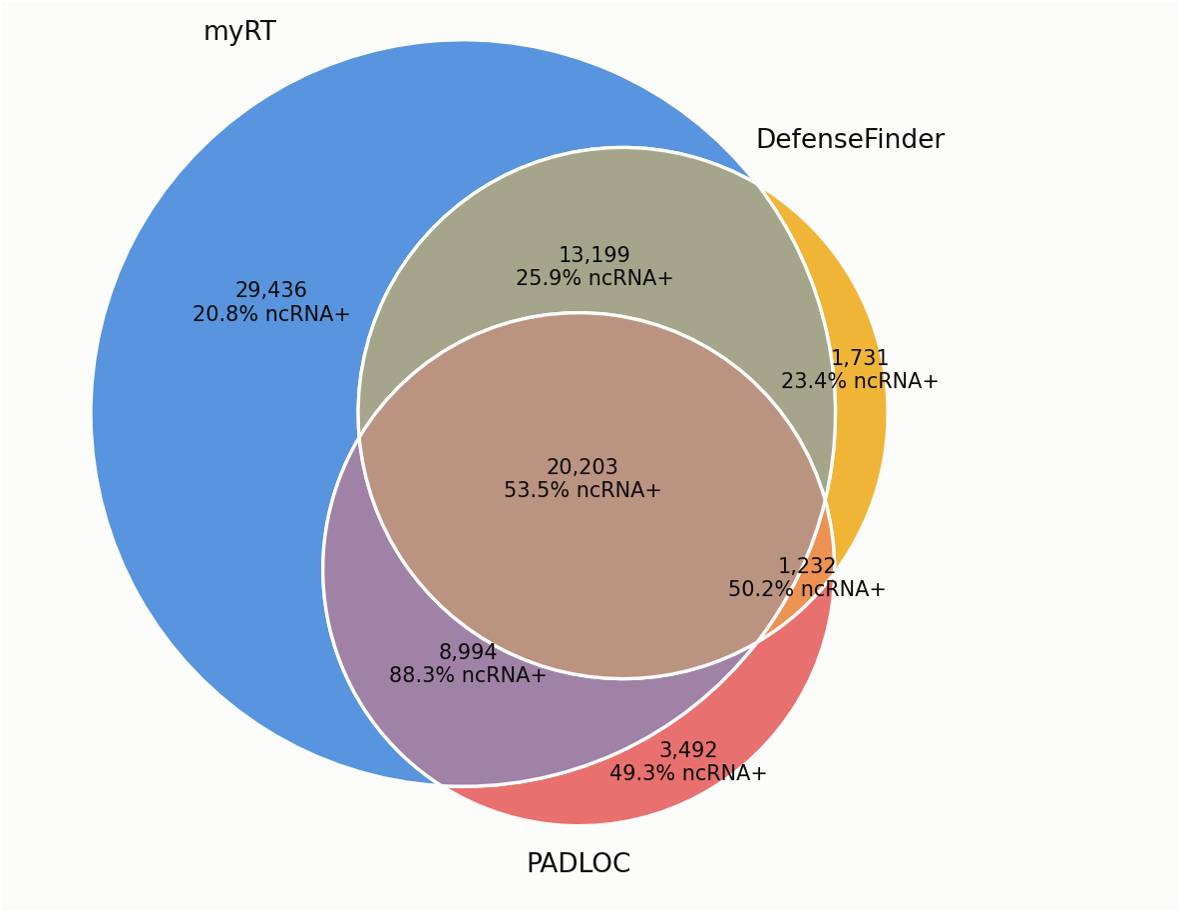
\includegraphics[width=\textwidth]{venn_diagram.png}
\caption[TBD]{TBD}
\label{fig:venn-diagram}
\end{figure}